% @Author: Mouna REKIK
% @Date:   2024-10-11 / 12:30
%%%%%%%%%%%%%%%%%%%%%%%%%%%%%%%%%%%%%%%%%%%%%%%%%%%%%%%%%%%%%%%%%%%%%%%%%%%%%%

\chapter{Contexte général du projet}
\begin{spacing}{1.2}
\minitoc
\thispagestyle{MyStyle}
\end{spacing}
\newpage

\section{Introduction}
Ce chapitre présente le cadre accueillant du projet, les bases théoriques et l’état de l’art liés aux systèmes conversationnels intelligents.
Nous commençons par exposer les approches existantes et leurs limites, afin de faire émerger la problématique centrale de notre projet.
Nous introduisons ensuite les concepts fondamentaux sur lesquels repose notre solution.

\section{Présentation du cadre du projet}
Dans cette section, nous présentons l’entreprise hôte, BACAB Consulting, ainsi que l’objectif général poursuivi dans le cadre de notre projet de fin d’études.
\subsection{Organisme d'accueil}
\subsubsection{Présentation}
Fondée en 2024, BACAB Consulting\cite{bacab-consulting} est une jeune startup composée d’une quinzaine de collaborateurs. Elle associe une expertise en stratégie d’entreprise à une maîtrise approfondie des technologies émergentes telles que le cloud computing et l’intelligence artificielle. Malgré sa création récente, la société s’engage à accompagner ses clients dans leur transformation numérique et analytique, en proposant des solutions cloud sécurisées et évolutives, ainsi que des systèmes intelligents conçus pour renforcer l’efficacité opérationnelle.\par
En suivant une culture d'excellence et d'innovation, BACAB Consulting encourage le développement continu des compétences de ses collaborateurs pour se positionner en tant que partenaire clé auprès de ses clients. En intégrant l’intelligence artificielle à ses offres, l’entreprise vise à renforcer sa valeur ajoutée, à instaurer une relation de confiance durable et à exploiter les données pour optimiser la prise de décision.
\begin{figure}[H]
    \centering
    
\includegraphics[height=3cm, keepaspectratio]{images/logo_bacab.png}
    \caption{Logo de BACAB Consulting \cite{bacab-consulting}}
    \label{bacab}
\end{figure}
\subsubsection{Secteurs d’activités}
BACAB Consulting intervient dans le domaine des technologies de l'information et concentre ses activités sur deux principaux volets :
\begin{itemize}[label=\textbullet]
    \item Cloud computing avec Microsoft Azure : L’entreprise accompagne ses clients dans la conception, le déploiement et l’administration de solutions cloud adaptées à leurs besoins. L’utilisation d’Azure permet d’exploiter tout le potentiel du cloud pour accélérer la croissance.
    \item Intelligence artificielle et recherche appliquée : En intégrant l’IA au cœur de ses projets, BACAB Consulting explore de nouvelles approches pour résoudre des problématiques complexes. L’entreprise propose des solutions modernes et intelligentes, capables d’automatiser des processus, d’optimiser les performances et d’offrir une aide précieuse à la décision stratégique.
\end{itemize}


\subsection{Objectif global}
L’objectif de ce projet est de concevoir et de mettre en place une plateforme complète permettant la gestion de chatbots personnalisés. Cette plateforme vise à offrir aux administrateurs la capacité de créer, modifier, supprimer et configurer des assistants virtuels, tout en leur permettant de s’adapter aux besoins spécifiques de leurs utilisateurs finaux. Ces derniers pourront ainsi interagir, via une interface conversationnelle, avec des agents alimentés par des règles et des actions sur mesure.\\
% La personnalisation des chatbots repose sur trois grands piliers:
% \begin{itemize}[label=\textbullet]
%     \item Intégration d’une base de connaissances: les assistants peuvent exploiter des documents importés (fichiers) ou des contenus web (\acs{URL}s), afin de répondre de manière précise et contextualisée aux questions des utilisateurs.
%     \item Utilisation de scénarios de questions-réponses: l’administrateur peut prédéfinir des paires questions/réponses considérées comme des règles métier ou des consignes prioritaires, ce qui garantit des réponses cohérentes et adaptées à des situations spécifiques.
%     \item Activation d’actions personnalisées: la plateforme permet de configurer des actions à exécuter, telles que l’appel d’une \acs{API} externe, l’envoi d’e-mails ou encore la recherche sur internet. Ces actions seront ensuite accessibles à l’agent, qui pourra les déclencher selon le contexte de la conversation.
% \end{itemize}
% En résumé, l’objectif de la plateforme est de permettre aux utilisateurs finaux de dialoguer avec des assistants \acs{IA} hautement spécifiés, configurés soit par eux-mêmes, soit par l’administrateur, tout en leur offrant un accès à des fonctionnalités avancées et à des sources de données actualisées.

\section{Étude de l’existant et problématique}
Dans cette section, nous présentons une analyse des principales solutions de création et de gestion de chatbots, leurs limites, ainsi que la problématique qui en découle.
\subsection{Étude de l'existant}
De nombreuses plateformes permettent aujourd’hui de concevoir, configurer et déployer des assistants conversationnels. Chacune cherche à se démarquer en élargissant les capacités de ses agents : compréhension de la demande de l'utilisateur, adaptation contextuelle rapide, accès à des bases de connaissances dynamiques, ou encore utilisation optimisée d’outils (recherche web, envoi d’e-mails, etc.). L’objectif commun est de couvrir un large éventail de cas d’utilisation tout en maintenant un haut niveau de précision, y compris dans des scénarios complexes.\par
Nous avons retenu trois plateformes représentatives :
\begin{itemize}[label=\textbullet]
    \item Rasa Studio : Rasa Studio est un outil no-code qui permet de créer, affiner et tester visuellement des assistants développés avec Rasa. Il offre à toute l’équipe, même aux membres n’ayant pas de compétences techniques avancées, la possibilité de concevoir des assistants et d'améliorer les contenus conversationnels, ainsi que de conduire des tests dans un même espace. Cette centralisation favorise la collaboration et simplifie le processus de développement d’agents conversationnels.
    \begin{figure}[H]
        \centering
        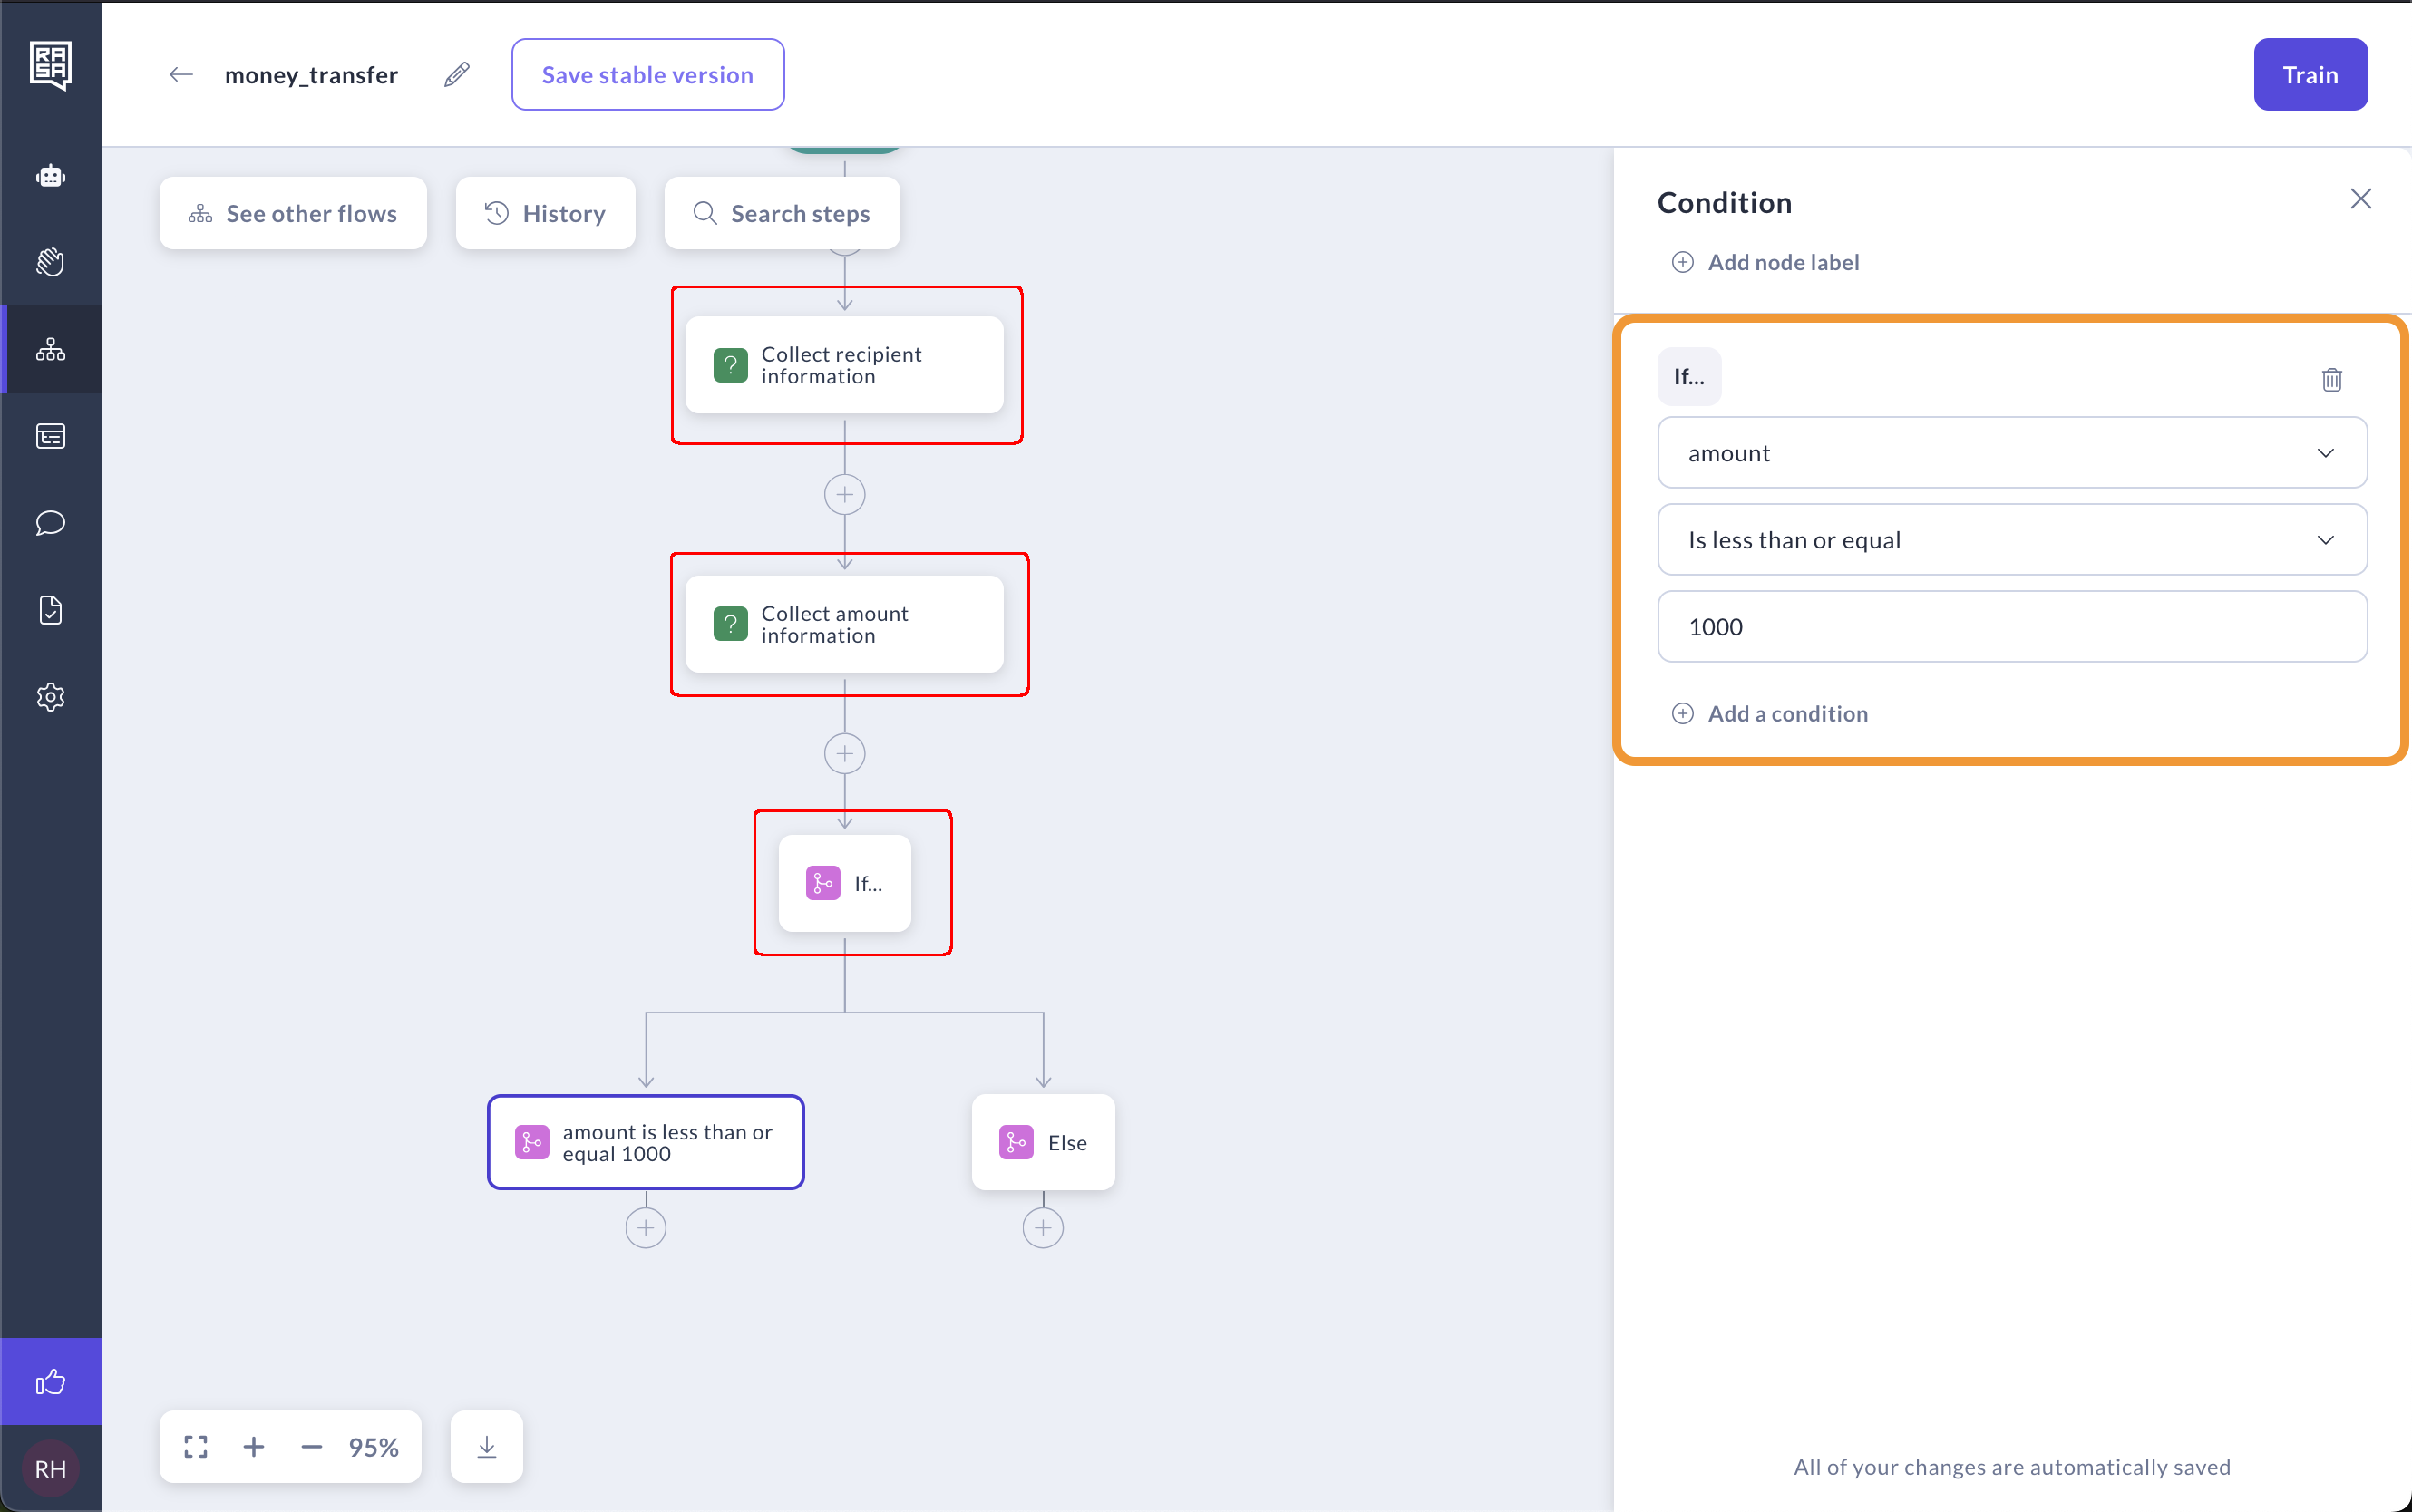
\includegraphics[height=7cm, keepaspectratio]{images/rasa_1 (1).png}
        \caption{Interface de création de flux dans Rasa Studio}
        \label{rasa1}
    \end{figure}
    Comme le montre la figure \ref{rasa1}, une des fonctionnalités essentielles de la plateforme est la configuration manuelle des flux conversationnels. L’administrateur peut définir pas à pas les réponses que l’agent devra fournir aux questions de l’utilisateur. Cette approche permet de guider la conversation vers un contexte bien déterminé, limitant ainsi la cohérence dans les scénarios contenant des questions imprévues.\\
    De plus, Rasa Studio offre la possibilité de configurer des actions personnalisées. Celles-ci permettent d’exécuter des traitements spécifiques, par exemple effectuer un calcul.
    \begin{figure}[H]
        \centering
        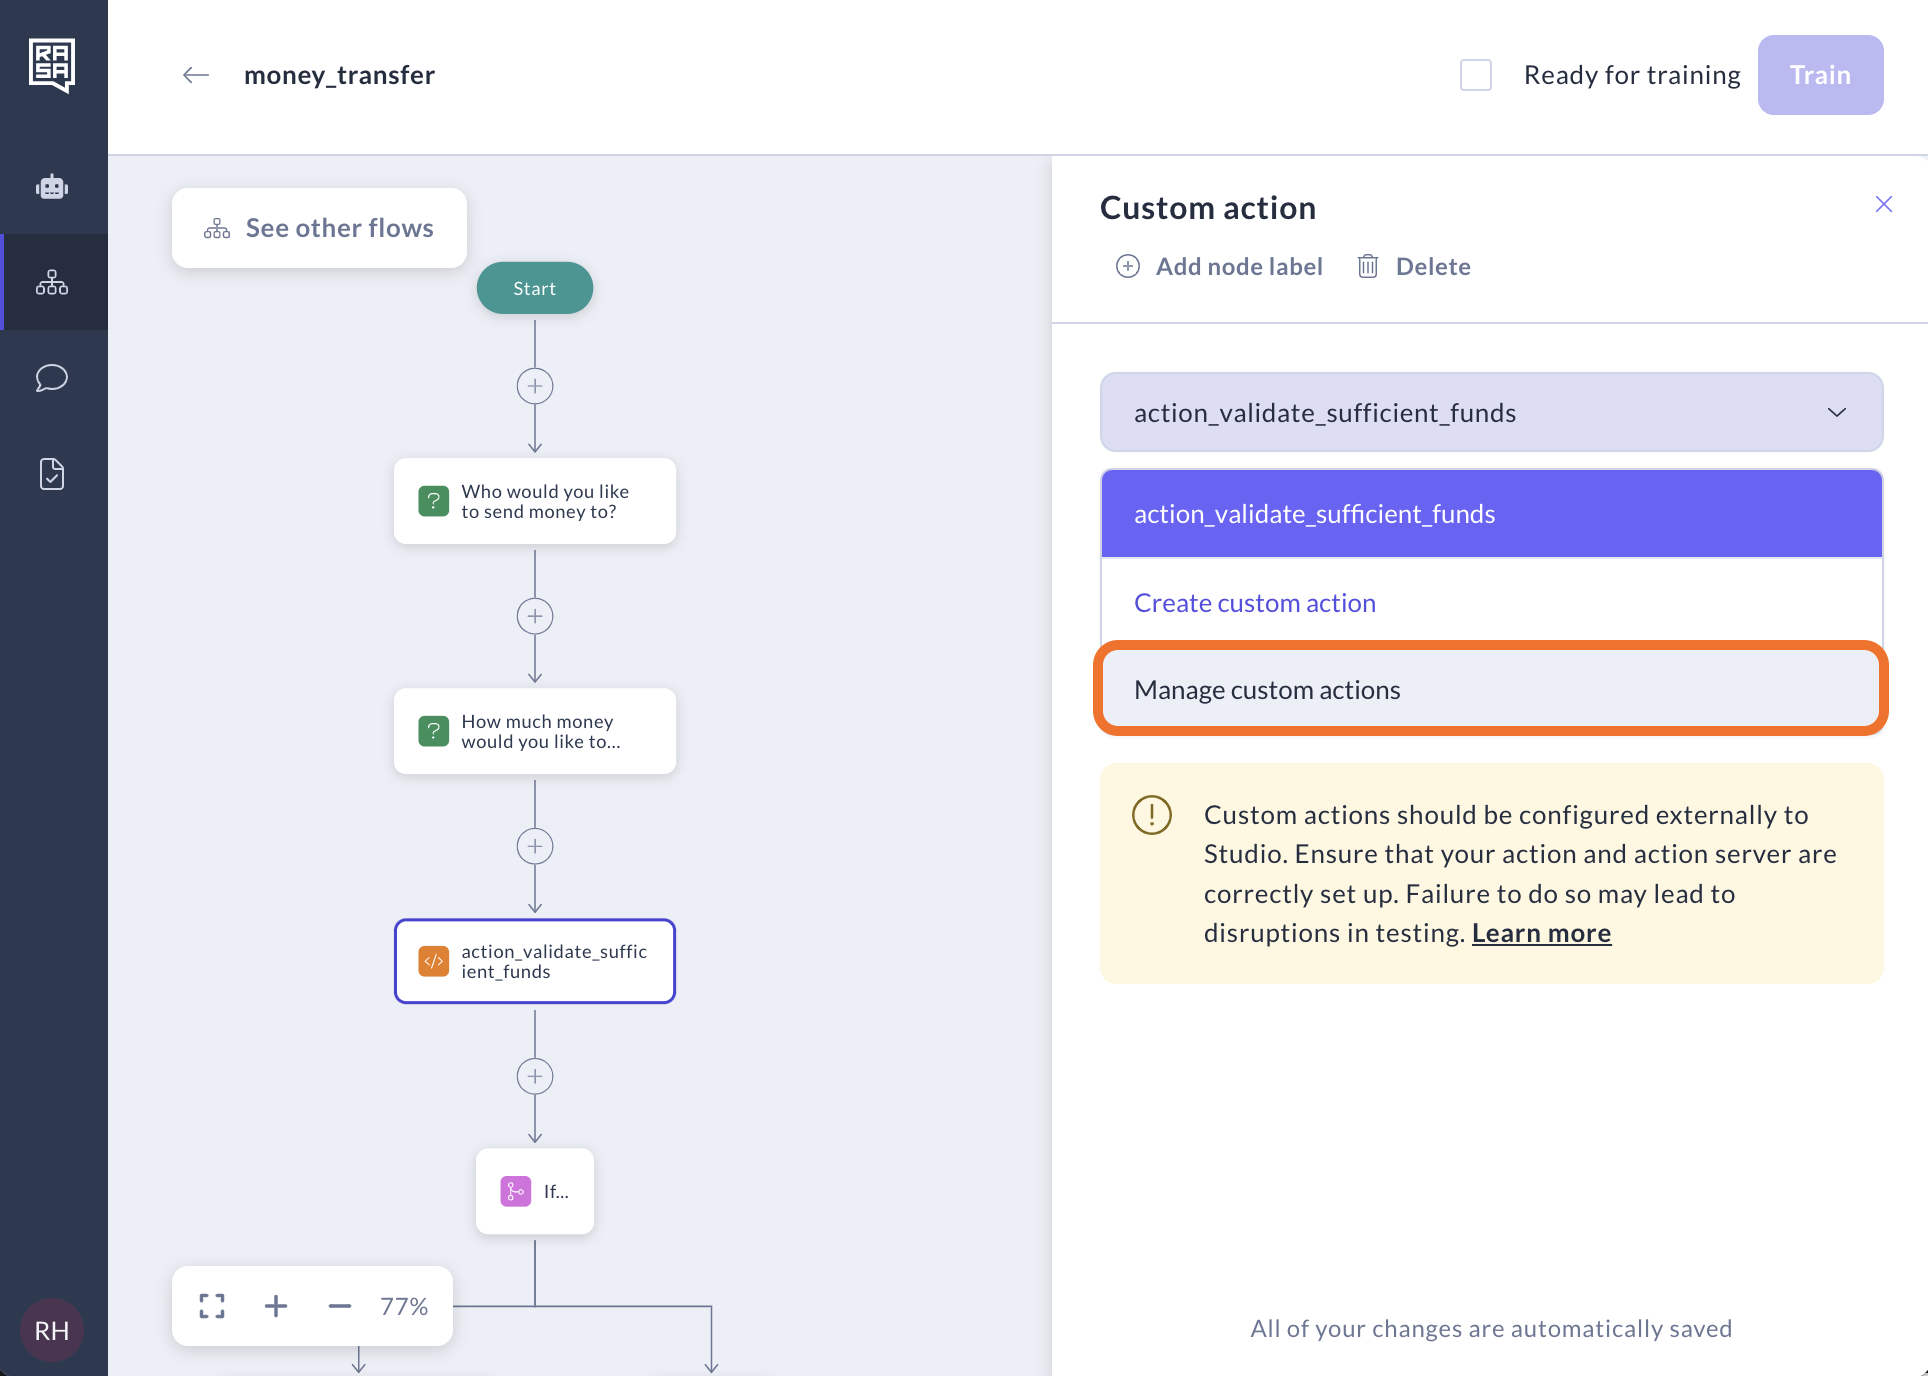
\includegraphics[height=7cm, keepaspectratio]{images/rasa_2.png}
        \caption{Exemple de configuration d'action}
        \label{rasa2}
    \end{figure}
    Toutefois, l’exécution de ces actions nécessite la mise en place d’un serveur externe qui héberge et exécute le code correspondant. La figure \ref{rasa2} illustre la configuration d’une action personnalisée, telle qu’un calcul de somme.
    \item Microsoft Copilot Studio (Microsoft Power Virtual Agents précédemment) : un outil graphique low-code qui permet de construire des agents et de définir leurs flux conversationnels. L’un de ses points forts réside dans sa capacité à se connecter à différents produits Microsoft grâce à des plugins préconstruits ou personnalisés. Cette flexibilité donne la possibilité aux utilisateurs de créer et d’orchestrer des logiques complexes.\\
    La figure suivante illustre l’interface principale de Copilot Studio, qui met à disposition de nombreux templates. Ces modèles couvrent différents cas d’usage (service client, finance, etc.) et peuvent être réutilisés directement, permettant ainsi aux administrateurs de démarrer rapidement sans tout configurer manuellement.
    \begin{figure}[H]
        \centering
        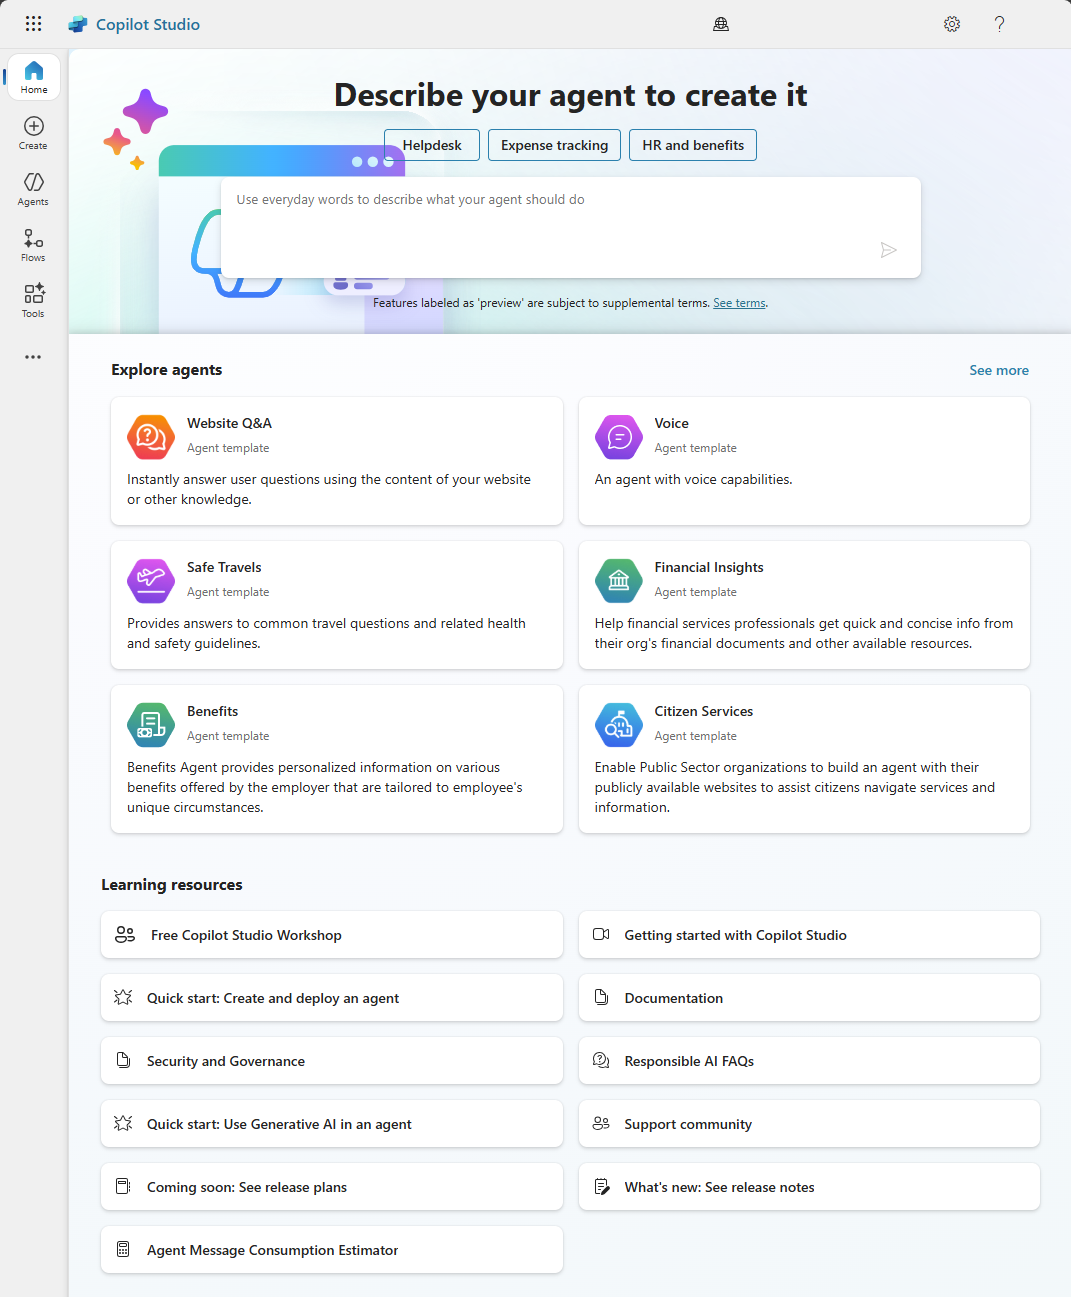
\includegraphics[height=8cm, keepaspectratio]{images/copilot.png}
        \caption{Interface principale de Copilot Studio}
        \label{copilot}
    \end{figure}
    En outre, la création d’un nouvel agent peut se faire directement depuis l’interface, comme le montre la figure ci-dessous.
    \begin{figure}[H]
        \centering
        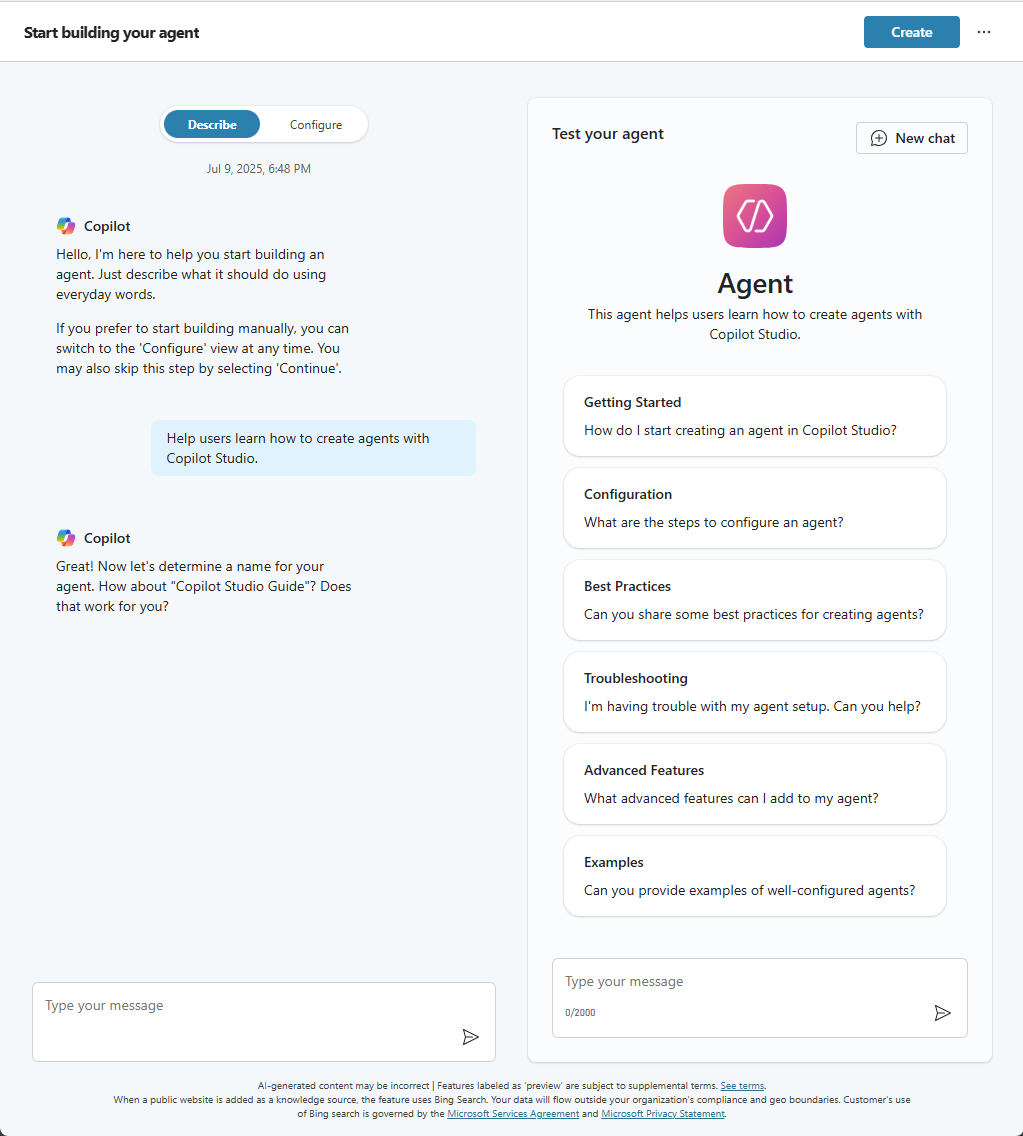
\includegraphics[height=8cm, keepaspectratio]{images/copilot_1.png}
        \caption{Interface de création d'agent dans Copilot Studio}
        \label{copilot1}
    \end{figure}
    La définition de l’agent se fait principalement par le biais d’une conversation guidée avec Copilot lui-même. L’utilisateur décrit son besoin en langage naturel, et Copilot propose progressivement une configuration adaptée. Cette approche est simple, mais elle présente une limite : les agents créés de cette manière sont moins adaptés aux scénarios nécessitant un contexte riche et persistant ou une mémoire conversationnelle étendue.
    \item ChatGPT : une plateforme proposant des modèles de langage (tels que GPT-5), orientée vers la génération de texte, la compréhension contextuelle et la conversation naturelle. Elle a connu une adoption massive grâce à une interface claire et révolutionnaire, permettant aux utilisateurs de poser des questions et d’obtenir rapidement des réponses cohérentes et pertinentes.\\
    Au fil du temps, de nouvelles fonctionnalités ont été ajoutées pour renforcer les capacités d'outils comme la recherche web, la génération et le téléchargement de fichiers, l’accès à des outils intégrés pour l’analyse de documents ou encore l’utilisation d’une mémoire conversationnelle permettant de mieux suivre les échanges. Ces évolutions en font un assistant polyvalent et performant, adapté à un large éventail d’usages.
    \begin{figure}[H]
        \centering
        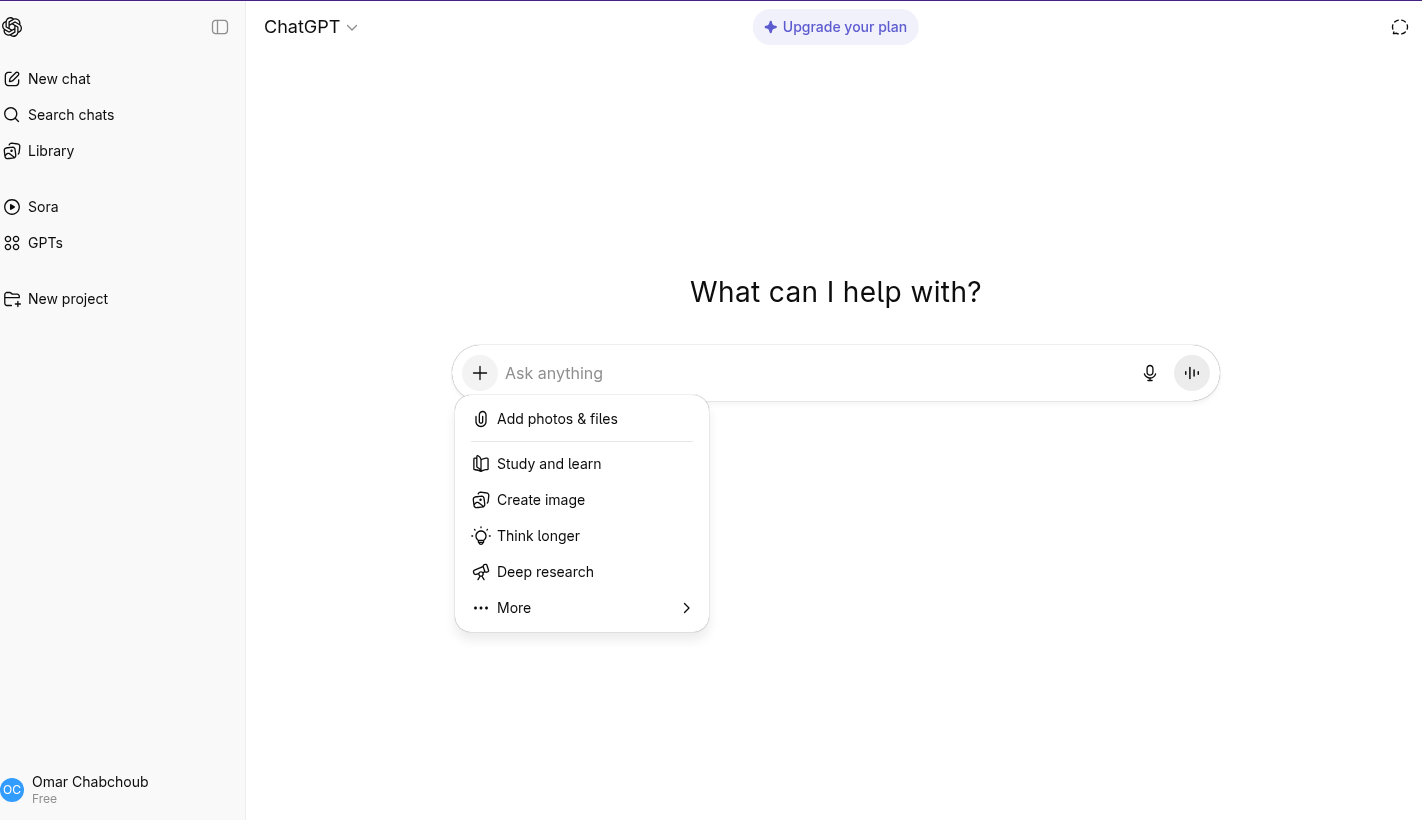
\includegraphics[height=8cm, keepaspectratio]{images/chatGPT.png}
        \caption{Interface de ChatGPT}
        \label{chatgpt}
    \end{figure}
    Cependant, malgré ses atouts, ChatGPT reste limité lorsqu’il s’agit de concevoir des chatbots entièrement personnalisés, car il ne propose ni gestion multi-agents, ni scénarios prédéfinis, ni intégrations poussées avec des systèmes métiers, ce qui le distingue des plateformes spécialisées comme Rasa Studio ou Microsoft Copilot Studio.
\end{itemize}
\subsection{Critique de l'existant}
Le tableau suivant compare les plateformes représentatives (Chatgpt, Rasa, Copilot), en illustrant aussi la valeur ajoutée de notre solution par rapport à l'existant.

\begin{table}[H]
\centering
\caption{Comparaison fonctionnelle des plateformes de chatbot}
\begin{tabular}{|>{\raggedright\arraybackslash}p{4cm}|
                >{\centering\arraybackslash}p{2.5cm}|
                >{\centering\arraybackslash}p{2.5cm}|
                >{\centering\arraybackslash}p{2.5cm}|
                >{\centering\arraybackslash}p{2.5cm}|}
\hline
\cellcolor{pastelgrey}\textbf{Critère} & 
\cellcolor{pastelgrey}\textbf{OpenAI ChatGPT} & 
\cellcolor{pastelgrey}\textbf{Rasa Studio} & 
\cellcolor{pastelgrey}\textbf{Microsoft Copilot Studio} & 
\cellcolor{pastelgrey}\textbf{Notre solution} \\ \hline

Accessibilité no-code & \xmark & \cmark & \cmark & \cmark \\ \hline
Support de base de connaissance & \xmark & \xmark & \cmark & \cmark \\ \hline
Actions personnalisées avancées & \xmark & \cmark & \xmark & \cmark \\ \hline
Gestion centralisée multi-agents & \xmark & \cmark & \cmark & \cmark \\ \hline
Intégration frontale & \xmark & \xmark & \cmark\footnotemark & \cmark \\ \hline
Connexion directe à documents/URLs & \xmark & \xmark & \cmark & \cmark \\ \hline
Extensibilité / modularité & \xmark & \cmark & \xmark & \cmark \\ \hline
Optimisé pour données multi-sources & \xmark & \xmark & \xmark & \cmark \\ \hline

\end{tabular}
\label{table:chatbot_comparison}
\end{table}
\footnotetext{L'intégration est limitée aux produits Microsoft.}

Le tableau \ref{table:chatbot_comparison} met en œuvre les différences essentielles entre les solutions populaires et notre propre plateforme, en considérant les critères suivants:

\begin{itemize}[label=\textbullet]

  \item \textbf{Accessibilité no-code} :  
  L’interface doit être \emph{user-friendly} et permettre à un administrateur non technique de créer et de configurer des chatbots sans écrire du code. Les actions doivent être effectuées à travers des formulaires simples, rendant la plateforme accessible à tous.

  \item \textbf{Support de base de connaissances} :  
  La plateforme doit offrir la possibilité d’importer différents types de fichiers (PDF, Word, CSV, pages web, etc.), sans limitation de nombre, afin de constituer une documentation de référence exploitable par le chatbot concerné.

  \item \textbf{Actions personnalisées avancées} :  
  L’utilisateur doit pouvoir définir facilement des actions en ajustant uniquement quelques paramètres. Par exemple, pour un appel API, il suffit de spécifier l’URL, les en-têtes et les paramètres, sans complexité technique.

  \item \textbf{Gestion centralisée multi-agents} :  
  Les différents assistants doivent être gérables de façon centralisée, tout en restant isolés. Chaque agent conserve son contexte, ses conversations et ses règles, permettant une supervision efficace sans interférence entre eux.

  \item \textbf{Intégration frontale} :  
  Le chatbot doit pouvoir être intégré dans des applications externes. Un \emph{widget}, par exemple, est une petite fenêtre interactive insérée dans un site web quelconque, permettant aux utilisateurs d’interagir avec le chatbot directement. L’administrateur du site peut ainsi déployer un agent dédié à ses visiteurs.

  \item \textbf{Connexion directe à documents et URLs} :  
  En complément des fichiers importés, il est utile de permettre la connexion à des sources en ligne (pages web, liens dynamiques). Cela assure que le chatbot accède toujours à une information actualisée sans devoir réimporter les données.

  \item \textbf{Extensibilité et modularité} :  
  L’architecture doit être conçue pour évoluer selon les cas d’usage. On doit pouvoir adapter ou enrichir les composants (par exemple, ajouter de nouveaux modules d’agents spécialisés) sans modifier tout le système existant.

  \item \textbf{Optimisation pour données multi-sources} :  
  La solution doit être capable de combiner efficacement plusieurs types de données (fichiers, URLs, bases externes). Cela permet de générer des réponses plus riches et adaptées aux contextes complexes.

\end{itemize}


\subsection{Problématique}
L’étude de l’existant a montré que, malgré leurs avancées, les solutions actuelles de création et de gestion de chatbots ne répondent pas totalement aux besoins combinant la flexibilité, la personnalisation et l'accessibilité pour des administrateurs non techniques. Elles restent limitées dans leur capacité à intégrer et exploiter de façon native des bases de connaissances issues de sources variées, à gérer plusieurs assistants de manière centralisée et modulaire, ou encore à prendre des décisions contextuelles complexes lors de la récupération et de l’utilisation des données.\\
Ces points mettent en évidence la nécessité d’une approche moderne, capable de surmonter les contraintes des plateformes traditionnelles tout en restant suffisamment accessible et évolutive pour des cas d’usage pratiques.
\section{Solution proposée}
Pour répondre à cette problématique, nous proposons une plateforme complète et simple.

D'une part, une base de connaissances flexible permettant l'importation de multiples fichiers de types variés, tels que des PDF pour des documents structurés, des CSV pour des données tabulaires ou des fichiers texte (TXT) pour des notes simples, tous indexés pour une récupération efficace sans grande limitation de nombre ou de taille, tout en intégrant des URLs dynamiques consultées en temps réel pour accéder à des informations actualisées et un module de questions-réponses (Q/R) préconfigurées où, si l'utilisateur pose une question correspondant sémantiquement à une entrée définie, l'assistant répond automatiquement avec la réponse associée, garantissant une cohérence et une personnalisation.

D'autre part, des actions sont configurables sans code via des formulaires clairs où l'administrateur choisit le type d'action, comme un appel REST API, un envoi d'e-mail ou une recherche web, en spécifiant des paramètres, tels que l'endpoint et les headers pour une API, et des conditions d'exécution simples, comme le déclenchement lors d'une demande utilisateur bien déterminée, assurant une intégration fluide dans les flux conversationnels. Ces actions servent à agrandir le potentiel de l'assistant pour consulter le maximum d'informations et répondre avec précision.

De plus, Le cadre administrateur offre une interface centralisée pour créer et gérer plusieurs assistants, en définissant leurs informations, comme le nom et le domaine d'application, leurs bases de connaissances, leurs actions personnalisées, leurs accès et permissions, chaque assistant restant modulaire et isolé pour une gestion optimale.

L'intégration est simplifiée grâce à des widgets, comme une bulle de conversation insérable sur un site web consommant l'API pour des interactions en temps réel, ou via des connecteurs vers des applications tierces comme WhatsApp, rendant le chatbot accessible dans divers environnements professionnels sans problème technique.

Notre solution se veut également adaptable et prête à incorporer divers outils d'IA en fonction des besoins spécifiques du domaine d'activité.

%Dans cette perspective, nous mettons particulièrement l’accent sur deux approches complémentaires que nous allons présenter : RAG (Retrieval-Augmented Generation) et l’approche agentique.

\section{Concepts de base}
La solution retenue dans notre projet repose sur des principes issus des avancées récentes en intelligence artificielle appliquée aux agents conversationnels, notamment la génération augmentée par la recherche (RAG) et l'approche agentique. Dans cette section, nous détaillons ces fondements. Nous commençons par les modèles de langage de grande taille (LLMs), en explorant leur évolution, leur fonctionnement, pour introduire les techniques d'optimisation telles que le prompting, le fine-tuning et le RAG, avant d'aborder l'approche agentique comme une extension puissante et autonome.

\subsection{Fondamentaux des LLMs}
\subsubsection{Définition}
Les modèles de langage de grande taille (LLMs) \cite{DL_book} représentent l'aboutissement d'une évolution rapide dans le domaine du traitement du langage naturel (NLP), un sous-domaine de l'intelligence artificielle qui vise à permettre aux machines de comprendre, générer et manipuler le langage humain de manière fluide et contextuelle. Le deep learning a favorisé cette progression en permettant aux réseaux neuronaux profonds d’apprendre à partir de grands corpus textuels. Ces réseaux seront ainsi capables de générer du langage sans nécessiter la programmation explicite de règles linguistiques.
\begin{figure}[H]
    \centering
    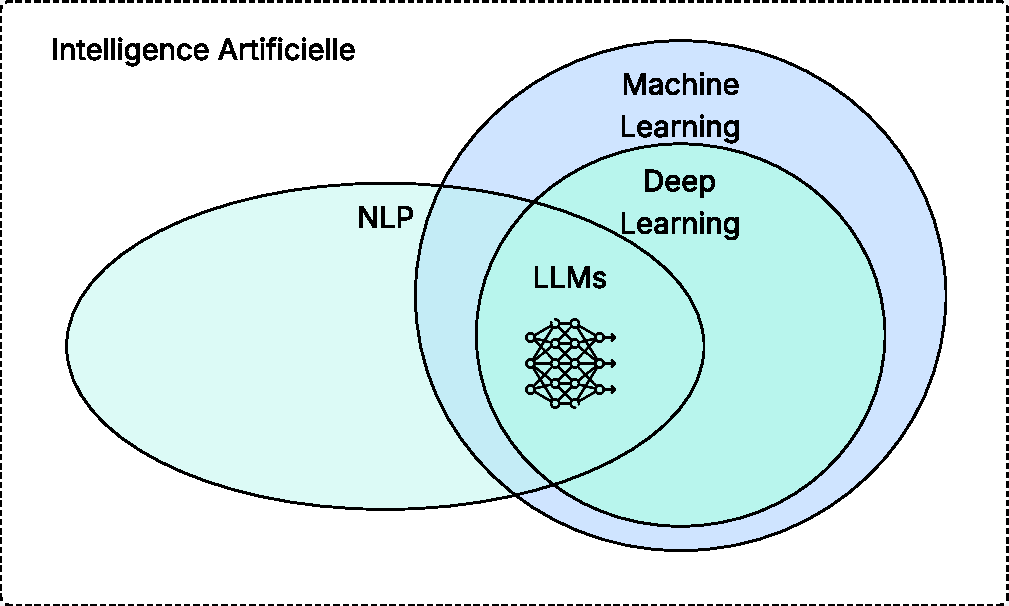
\includegraphics[height=8cm, keepaspectratio]{images/Figure AI-ML-DL-LLMs.pdf}
    \caption{Positionnement des LLMs dans les domaines d'IA}
    \label{fig:ai-llm}
\end{figure}
Pour mieux comprendre d’où viennent les LLMs, au départ, dans les années 1950-1960, les ordinateurs utilisaient des approches simples basées sur des règles fixes, comme des dictionnaires ou des grammaires codées à la main. Ces systèmes, bien que fonctionnels pour des tâches limitées, étaient rigides et incapables de s’adapter à de nouveaux contextes. Une percée survient avec les modèles statistiques dans les années 1980-1990, comme les n-grammes \cite{manning1999foundations}, qui prédisaient les mots suivants dans une phrase en se basant sur des probabilités calculées à partir de grands textes. Par exemple, si le texte contient souvent « le chat dort », un n-gramme pourrait suggérer « dort » après « le chat ». Cependant, ces modèles restaient limités à de courtes séquences et manquaient de compréhension profonde.
\begin{figure}[H]
\centering
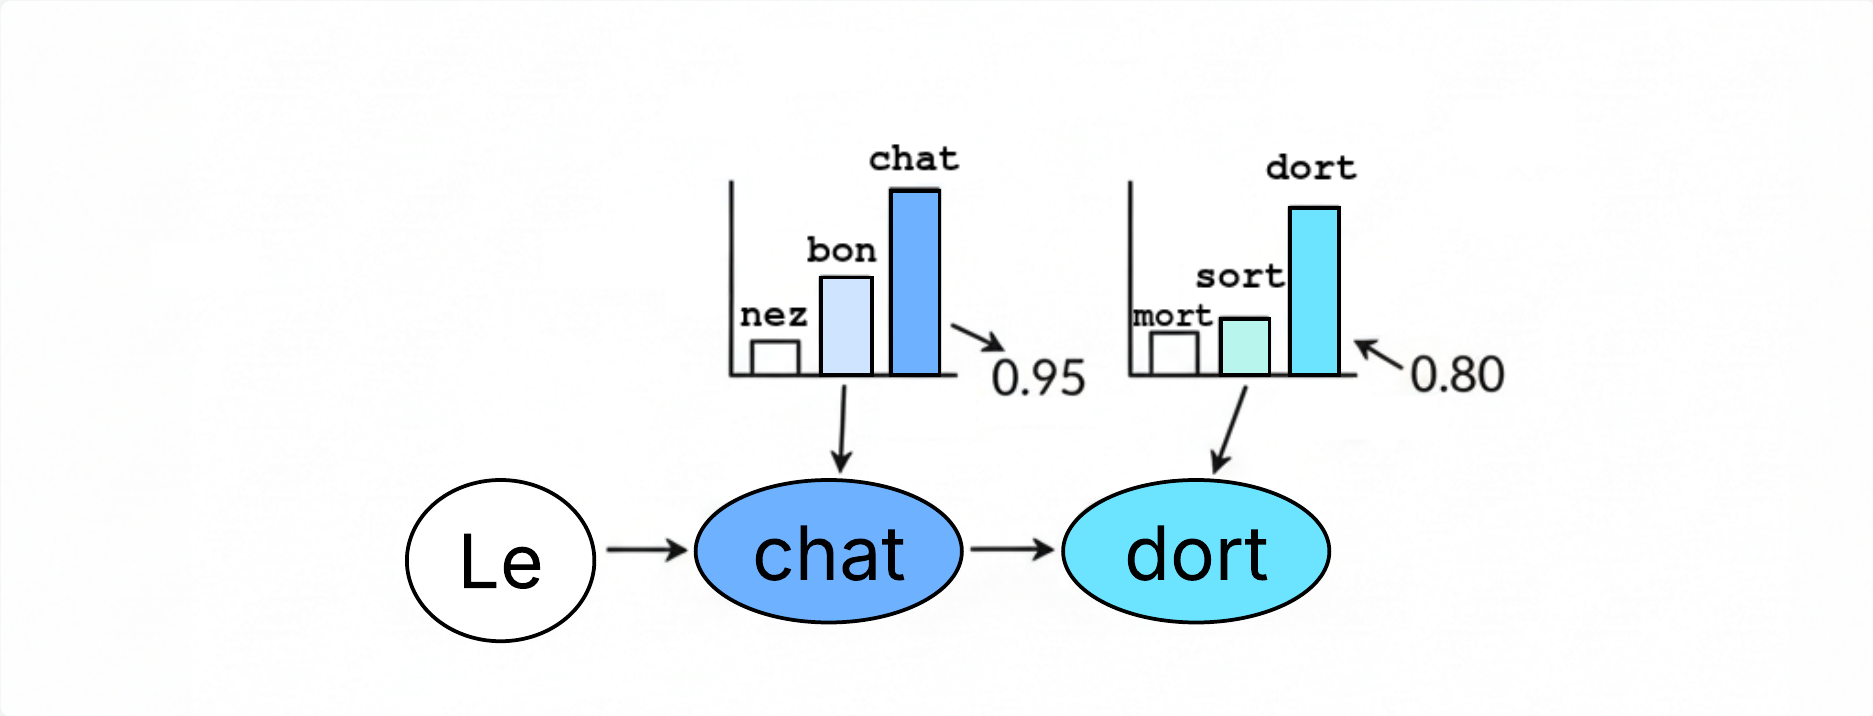
\includegraphics[width=1\linewidth, keepaspectratio]{images/n-grams.png}
\caption{Exemple simplifié d’un modèle n-gramme}
\label{fig:ngram}
\end{figure}
Ensuite, dans les années 2000, les réseaux neuronaux récurrents (RNN) \cite{elman1990finding} ont introduit une mémoire séquentielle, permettant aux machines de « se souvenir » des mots précédents dans une phrase. Mais ces RNN avaient un défaut : ils ne gèrent pas bien les longues phrases, car l’information s’affaiblissait au fil du temps, un problème appelé « disparition du gradient ». Par exemple, dans un paragraphe, le modèle a du mal à conserver le lien avec les premiers mots: le contexte initial s’atténue progressivement.\\
Pour surmonter cette limite, des variantes comme les LSTM (Long Short-Term Memory) et les GRU (Gated Recurrent Unit) ont été développées. Les LSTM utilisent des portes (forget, input, output) pour contrôler ce qui est mémorisé ou oublié, comme une sorte de filtre intelligent qui retient les informations importantes sur de longues périodes \cite{hochreiter1997long}. Les GRU, plus simples, combinent deux portes (input, forget) en une seule unité, offrant une alternative efficace mais moins flexible \cite{chung2014empirical}. Malgré ces améliorations, ces architectures restent lentes à entraîner sur de très longues séquences et peuvent encore souffrir de goulets d’étranglement computationnels ou d’oubli partiel dans des contextes très complexes.
\begin{figure}[H]
\centering
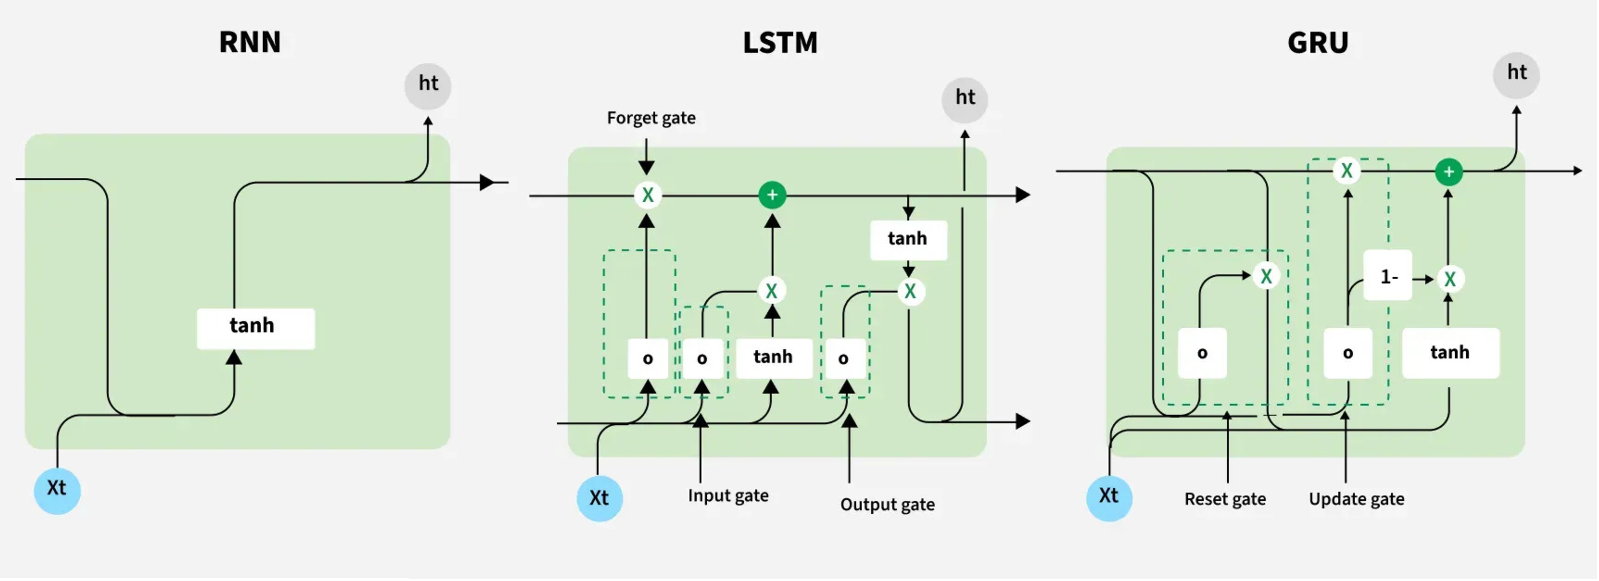
\includegraphics[width=1\linewidth, keepaspectratio]{images/rnn_lstm_gru.pdf}
\caption{Évolution de la structure de base d'un RNN \cite{rnn-lstm-gru}}
\label{fig:rnn-lstm-gru}
\end{figure}
La révolution arrive en 2017 avec les transformers \cite{vaswani2017attention}, une architecture qui traite toutes les parties d’une phrase en même temps, comme si chaque mot « observait » tous les autres pour comprendre le contexte global.
\begin{figure}[H]
\centering
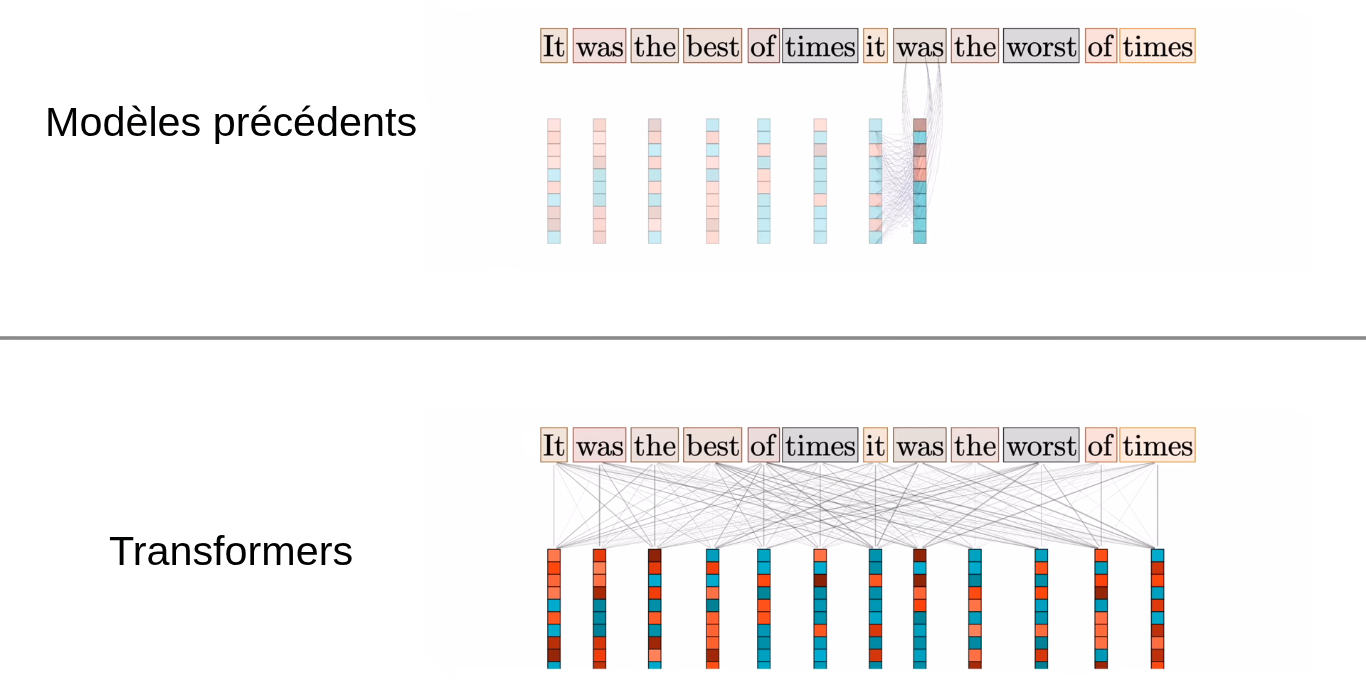
\includegraphics[width=1\linewidth, keepaspectratio]{images/transformers.png}
\caption{Traitement des mots avec Transformers}
\label{fig:transformers}
\end{figure}
La figure \ref{fig:transformers} montre bien comment les transformers ne lisent pas le texte de manière linéaire de début à la fin, mais l’absorbent en totalité en parallèle grâce à un mécanisme appelé "attention".
Cela a permis des modèles plus puissants et rapides. Les LLMs, comme GPT ou BERT, amplifient cette idée en entraînant des transformers sur des quantités énormes de textes – des milliards de mots issus d’internet ou de livres – pour capturer des significations complexes et générer des réponses semblables à celles d’un humain.
Le tableau suivant résume la comparaison effectuée à travers l’évolution architecturale des modèles étudiés:
\begin{table}[H]
    \caption{Comparaison des architectures de traitement du langage}
    \centering\resizebox{\linewidth}{!}{
    \label{tab:architecture_comparison}
    \begin{tabular}{|l|l|l|l|l|}
        \hline
        \textbf{Paramètre} & \textbf{RNN} & \textbf{LSTM} & \textbf{GRU} & \textbf{Transformers} \\
        \hline
        \textbf{Architecture} & Boucles simples & Cellules avec portes & Portes simplifiées & Mécanisme d’attention \\
        \hline
        \textbf{Longues séquences} & Faible (gradient) & Bonne & Modérée & Excellente \\
        \hline
        \textbf{Temps d’entraînement} & Rapide & Lent & Moyen & Intensif (parallèle) \\
        \hline
        \textbf{Mémoire} & Faible & Élevée & Moyenne & Très élevée \\
        \hline
        \textbf{Parallélisme} & Limité & Limité & Limité & Élevé \\
        \hline
    \end{tabular}}
\end{table}
\subsubsection{Fonctionnement général}
Le fonctionnement d’un LLM repose sur un processus itératif et probabiliste, où l’entrée textuelle est transformée en une représentation numérique, traitée par l’architecture du transformer, puis convertie en sortie générée. Au cœur de ce mécanisme se trouve la tokenisation, qui divise le texte en unités élémentaires appelées jetons.\par
% \paragraph{Les jetons}
Un jeton ou "token" \cite{openai_tokens} désigne l’unité élémentaire de traitement du texte. Il ne correspond pas nécessairement à un mot entier : il peut s’agir d’un mot, d’une partie de mot, d'un caractère ou encore d’un mot suivi d’un espace. Avant d’être analysé par le modèle, le texte est découpé en une séquence de jetons, selon une segmentation spécifique qui ne coïncide pas toujours avec les frontières naturelles des mots.
\begin{figure}[H]%
    \center%
    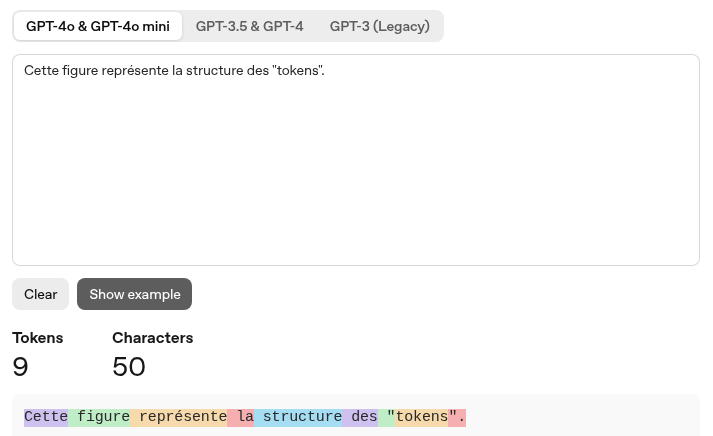
\includegraphics[width=\textwidth, keepaspectratio]{images/capture_tokens.png}%
    \caption{Les tokens dans un texte}%
\end{figure}
Cette étape est importante, car elle détermine la fenêtre de contexte, c’est-à-dire un nombre maximal de jetons qu’un modèle peut traiter à la fois, incluant à la fois l’entrée (la requête) et la sortie (la réponse générée). Cette limite varie selon la version du modèle. Par exemple, certains modèles récents peuvent gérer jusqu’à 32 000 voire 128 000 tokens en une seule séquence.
Lorsque cette limite est atteinte, le modèle ne peut plus prendre en compte les jetons excédentaires. Cela peut entraîner une perte d’information contextuelle ou empêcher la génération de réponses complètes. Pour optimiser les performances, il est donc essentiel de gérer efficacement la longueur des requêtes et des réponses, et, si nécessaire, de résumer ou découper le contenu.\par
En termes d’entrées et sorties, l’input est le prompt – une instruction ou un contexte fourni par l’utilisateur – tandis que l’output est la génération autoregressive, où chaque nouveau jeton dépend des précédents. C’est précisément pour optimiser cet input-output que le prompt engineering émerge comme une technique clé, transformant la formulation du prompt en une ingénierie méthodique pour améliorer la qualité de l’output sans modifier le modèle.
\subsubsection{Prompt engineering et ses techniques}
\paragraph{Définition}
Le prompting ou de manière plus avancée, le “prompt engineering” \cite{liu2023pre} désigne l’art de formuler une instruction ou une entrée destinée à guider le comportement d’un modèle de langage lors de la génération d’une réponse. Dans les modèles comme GPT, le prompt joue un rôle central, car il définit le contexte à partir duquel le modèle va prédire la suite de texte la plus probable. Ainsi, un même modèle peut accomplir une grande variété de tâches selon la manière dont le prompt est rédigé.

\paragraph{Techniques}
\subparagraph{Prompting direct ou Zero-shot prompting}
Le zero-shot prompting \cite{radford2019language} représente une nouvelle approche dans l'utilisation des grands modèles de langage (LLMs). Contrairement aux méthodes traditionnelles nécessitant de vastes ensembles de données annotées, cette technique repose sur la bonne formulation de consignes et d’instructions permettant au modèle de réaliser des tâches inédites. Ce dernier reçoit ainsi une description de la tâche à accomplir, sans disposer d'exemples d’apprentissage spécifiques associant des entrées à des sorties. Il s'appuie sur ses connaissances préalablement acquises pour produire des réponses pertinentes en fonction de l'instruction fournie.\\
Par exemple, pour classer un texte comme positif ou négatif, un prompt simple pourrait être : « Classifie le sentiment de cette phrase : 'Ce film est génial !' ». Le LLM, sans exemple préalable, infère la tâche et répond : « Positif ». 
\begin{figure}[H]%
    \center%
    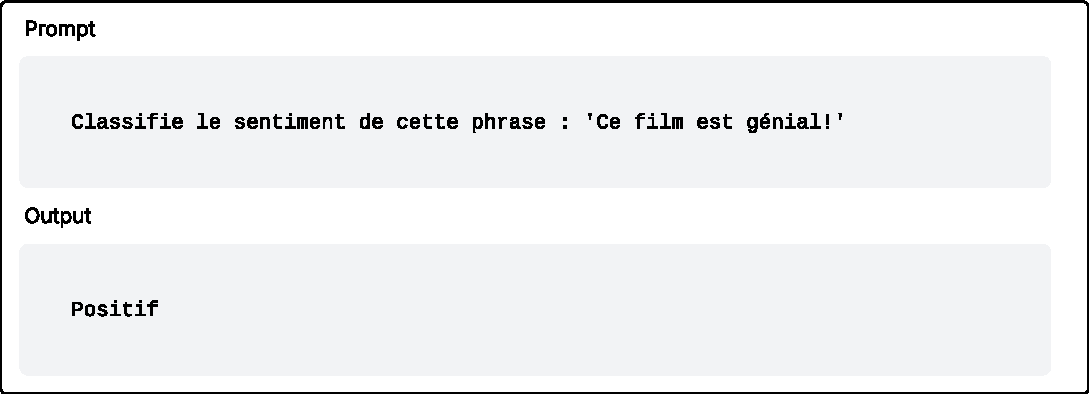
\includegraphics[width=\textwidth, keepaspectratio]{images/zero-shot.pdf}%
    \caption{Exemple de zero-shot prompting}%
\end{figure}
Cette approche est efficace pour des tâches générales, mais peut manquer de précision sur des domaines spécialisés, où le modèle risque des généralisations erronées.

\subparagraph{Few-shot prompting}
Le few-shot prompting \cite{brown2020language} consiste à fournir au modèle quelques exemples d’entrées et de sorties afin de lui permettre de comprendre la tâche à accomplir, contrairement au zero-shot prompting, qui ne repose sur aucun exemple. Même un petit nombre d’exemples bien choisis peut considérablement améliorer les performances du modèle, notamment pour des tâches complexes.\\
Prenons le même exemple de classification : le prompt inclut maintenant des démonstrations : « Exemple 1 : 'J'adore ce livre.' → Positif. Exemple 2 : 'C'est nul.' → Négatif. Classifie : 'Ce film est génial !' ». Le modèle répond plus fidèlement : « Positif », en imitant le pattern observé. Cette technique excelle pour des tâches nuancées, comme la traduction stylée ou l'analyse sémantique.\\
\begin{figure}[H]%
    \center%
    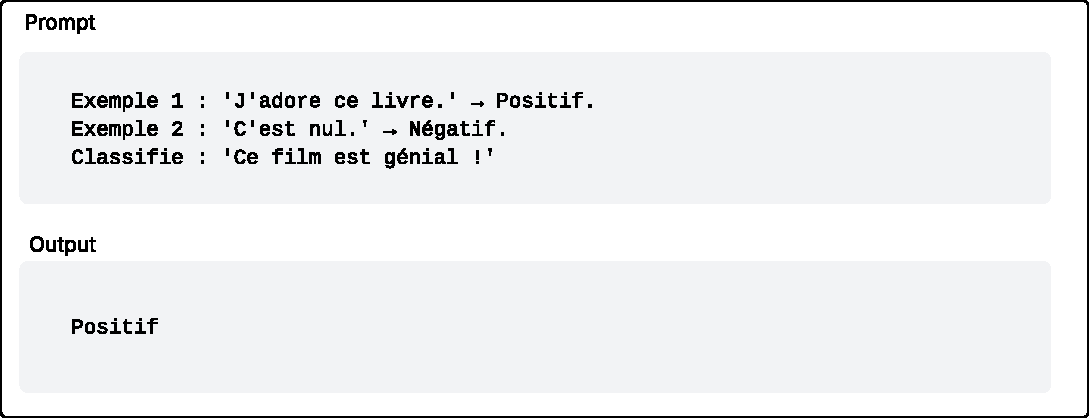
\includegraphics[width=\textwidth, keepaspectratio]{images/few-shot.pdf}%
    \caption{Exemple de few-shot prompting}%
\end{figure}
Toutefois, cette méthode nécessite l’ajout de jetons (Tokens) supplémentaires, ce qui peut devenir contraignant lorsque les textes à traiter sont longs. De plus, la sélection et la structuration des exemples influencent fortement le comportement du modèle. Certains biais, tels que la préférence pour les mots fréquents, peuvent également persister.

\subparagraph{Chain-of-thought prompting}
Les grands modèles de langage (LLMs) rencontrent encore des difficultés lorsqu’ils sont confrontés à des questions nécessitant un raisonnement complexe, ce qui limite leur potentiel. Pour répondre à cette limitation, la méthode du Chain-of-Thought prompting (CoT) \cite{wei2022chain} est une technique inventée pour raisonner de manière plus structurée et progressive.\par
L'apport principal de cette approche réside dans la formulation de consignes (prompts) qui encouragent le modèle à suivre une chaîne logique d’étapes intermédiaires, plutôt qu’à fournir une réponse immédiate. Cette méthode permet d’obtenir des réponses plus cohérentes et proches du raisonnement humain.\par
En effet, plusieurs expériences démontrent l’efficacité de cette technique, notamment en l’appliquant à des problèmes mathématiques complexes ou à des questions de raisonnement. Par exemple, au lieu de demander directement une réponse finale, le prompt présente une résolution étape par étape, imitant ainsi la manière dont une personne décomposerait un problème en sous-étapes.

\begin{figure}[H]%
    \center%
    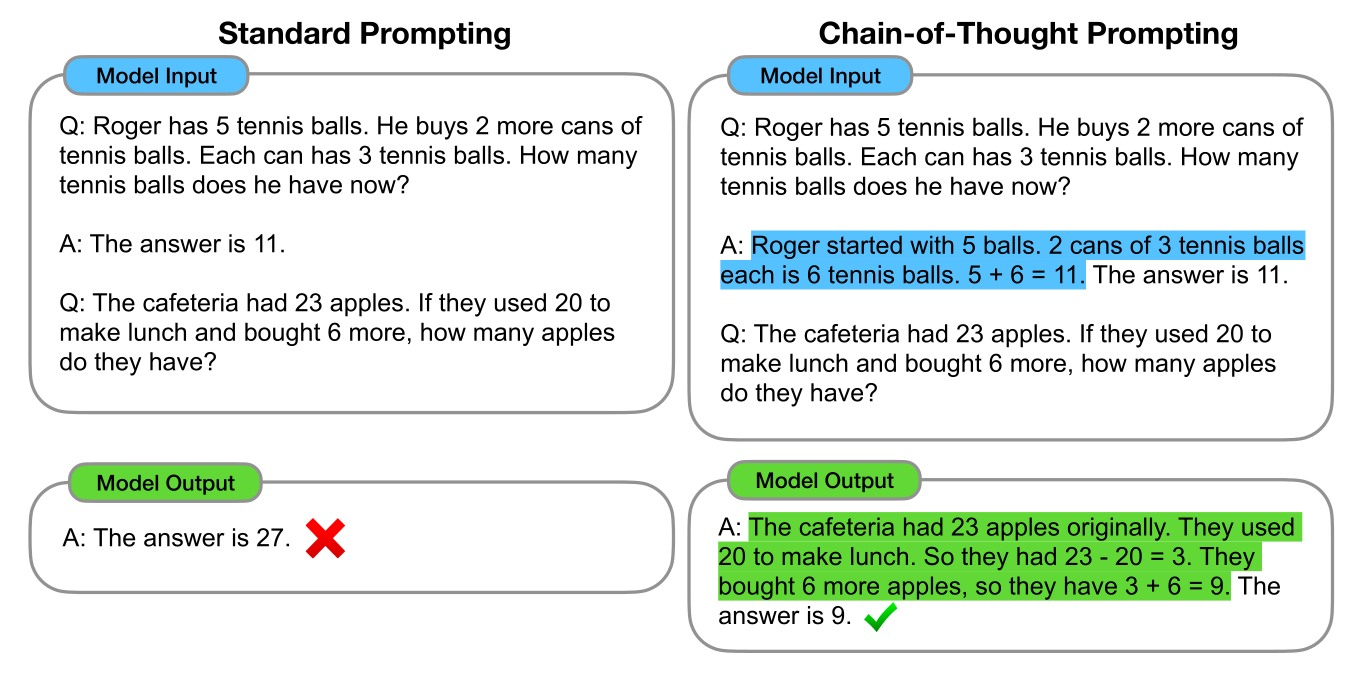
\includegraphics[width=\textwidth, keepaspectratio]{images/capture_CoT.png}%
    \caption{L'impact de CoT sur le raisonnement\cite{wei2022chain}}%
\end{figure}

Cette figure compare deux approches de prompting sur des problèmes arithmétiques simples. À gauche, le prompting standard (correspondant au few-shot) montre le modèle donnant des réponses directes sans explication, aboutissant à des erreurs (comme la réponse incorrecte "27" marquée d'une croix rouge). À droite, le Chain-of-Thought Prompting présente le même modèle décomposant explicitement chaque étape du raisonnement, ce qui a conduit à une réponse correcte et vérifiable.\par

\subsubsection{Personnalisation des LLMs}
Bien que les LLMs soient extrêmement performants, leurs connaissances sont limitées aux données statiques de leur entraînement, qui peuvent devenir obsolètes au fil du temps ou ne pas couvrir des domaines particuliers.\par
Dans le cadre de notre projet, l'objectif est de personnaliser ces modèles pour des chatbots adaptés à des bases de connaissances dynamiques et variées. Une approche classique pour y parvenir est le fine-tuning, qui consiste à réentraîner un LLM pré-entraîné sur un jeu de données (datset) ciblé afin d'ajuster ses poids pour un domaine particulier.\par
Ses avantages incluent une spécialisation précise et une réduction des hallucinations dans le contexte visé pour générer des réponses personnalisées à un secteur d'activité donné. Cependant, le fine-tuning présente des inconvénients majeurs : il est coûteux en ressources computationnelles (nécessitant souvent des GPU haut de gamme et des heures d'entraînement) et manque de flexibilité pour des mises à jour fréquentes, car chaque changement nécessite un nouveau réentraînement complet.\par
C'est pourquoi la génération augmentée par la recherche (Retrieval-Augmented Generation, ou RAG) a révolutionné la personnalisation des LLMs. Contrairement au fine-tuning, qui modifie le modèle lui-même, le RAG conserve la polyvalence du LLM tout en l'enrichissant dynamiquement avec des informations récupérées d'une base de connaissances externe. Cela lui permet d'accéder à des données actualisées ou privées sans réentraînement, évitant les coûts prohibitifs.

\subsection{Aperçu sur le RAG}
Rappelons que notre objectif de développer une plateforme de chatbots personnalisables et accessibles, capable d'exploiter des bases de connaissances dynamiques et multi-sources (fichiers PDF, CSV, URLs, etc.). Le RAG émerge comme une solution idéale pour surmonter les limites des LLMs, telles que les "hallucinations".\\
Ce terme désigne des affirmations linguistiquement correctes, semblant crédibles, mais qui sont actuellement erronées, inventées ou non fondées sur une source réelle. Ces hallucinations surviennent lorsque le modèle tente de répondre à des questions qui dépassent son champ de connaissances ou pour lesquelles il n’existe pas de réponse fiable dans ses données d’entraînement.
\subsubsection{Fonctionnement du RAG}
Le RAG (Retrieval-Augmented Generation) combine les capacités de raisonnement d’un LLM (Generator) avec un module de récupération d’informations externes (Retriever)\cite{lewis2020retrieval}. Son principe repose sur un pipeline modulaire : avant de générer une réponse, le système interroge une base documentaire (souvent vectorielle), récupère les passages les plus pertinents, puis les injecte dans le prompt du modèle. Celui-ci peut alors s’appuyer sur un contexte à jour et actualisé pour formuler sa réponse. En d’autres termes, le concept "RAG" est devenu la manière standard de faire fonctionner l’IA générative sur ses propres données.\par
\begin{figure}[H]%
    \centering
    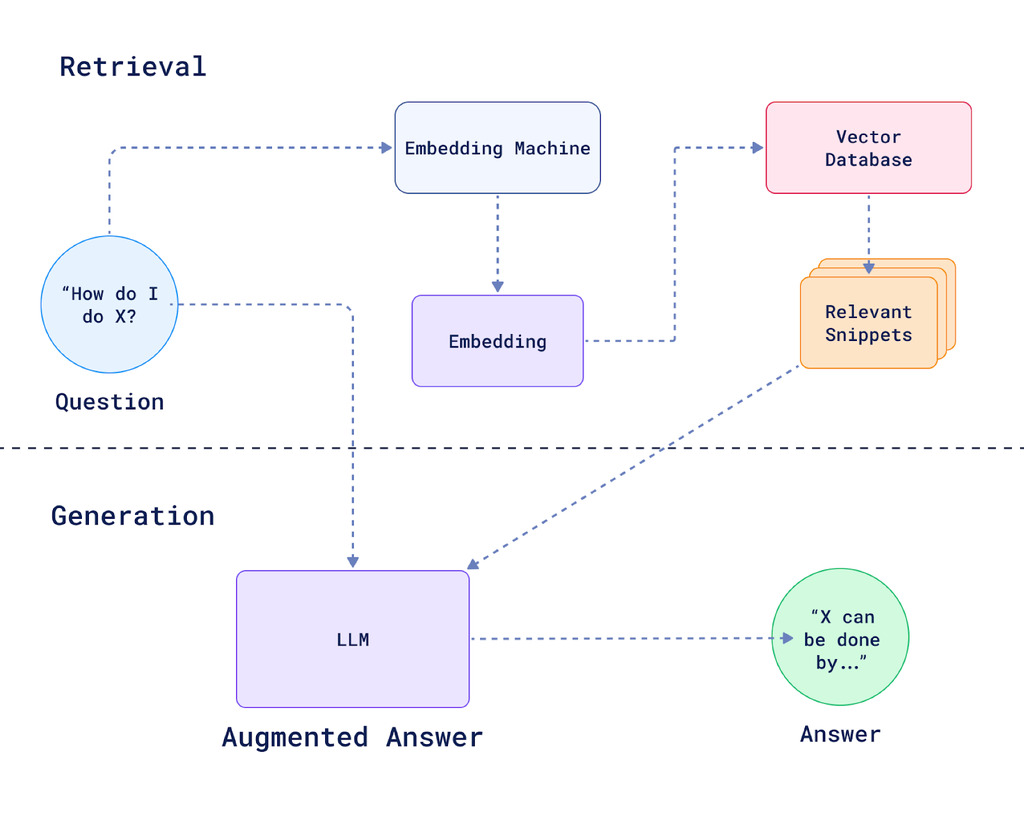
\includegraphics[height=9cm, keepaspectratio]{images/retrv_gen.jpg}%
    \caption{Architecture du système RAG avec les phases de récupération et de génération\cite{qdrant2024rag}}%
    \label{fig:arch_rag}
\end{figure}
La figure \ref{fig:arch_rag} illustre un parcours bien tracé d'une question ainsi que la génération de sa réponse: elle commence par la phase de récupération, où elle est transformée en une représentation (Embedding) via le modèle responsable (Embedding Machine). Cette représentation est ensuite explorée dans la base  de connaissance (Vector Database), où les passages adéquats (Relevant Snippets) sont sélectionnés et ajoutés à la question. Ces éléments enrichis alimentent ensuite le modèle (LLM) pour émettre une réponse claire dans la phase de génération.

Ce processus s'articule en étapes interconnectées, alignées sur notre plateforme pour une personnalisation efficace :
\paragraph{Ingestion et structuration des données}
Avant que le pipeline ne démarre, les données sont préparées lors d’une étape d’ingestion, qui alimente la base initiale (Vector Database sur la figure~\ref{fig:arch_rag}). Cette étape est effectuée une seule fois, mais elle peut être répétée lors de l’ajout de nouvelles sources. Le pipeline lui-même utilise ensuite ces données structurées pour la suite du traitement.

Cette phase débute par la collecte et la préparation des sources de données : fichiers (PDF, CSV, DOCX), textes, contenus extraits de sites web, etc. Ces documents sont chargés et transformés si nécessaire (parsing), puis découpés en segments textuels (splitting). Ces segments sont appelés chunks. Ce niveau de granularité facilite une gestion efficace des connaissances dans le RAG, en évitant de surcharger le contexte du LLM avec des documents entiers, tout en préservant la cohérence sémantique pour une récupération précise.
\begin{figure}[H]
\centering
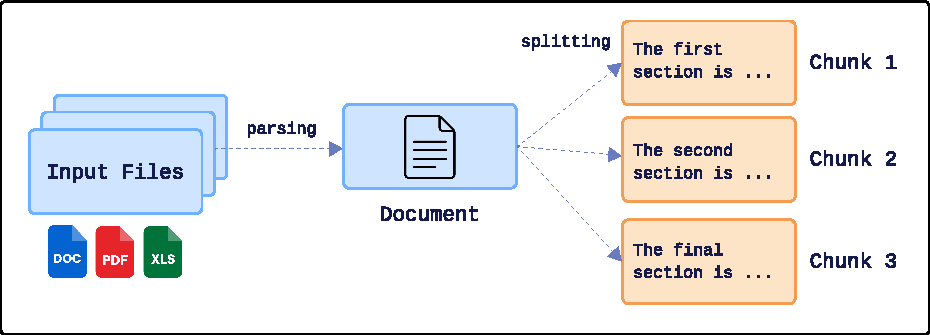
\includegraphics[width=1\linewidth, keepaspectratio]{images/inject.pdf}
\caption{Transformation des fichiers en segments via découpage}
\label{fig:injection_rag}
\end{figure}
Les paramètres de découpage (splitting) jouent un rôle primordial dans l'efficacité des segments récupérés. En découpant en chunks (généralement 200-500 mots), nous limitons la taille du contexte injecté dans le LLM. Par conséquent, nous respectons sa fenêtre de tokens et nous améliorons la précision de la recherche en isolant des idées spécifiques. Un découpage trop grossier perd des détails, tandis qu’un découpage trop fin casse la cohérence ; un chevauchement (overlap) entre chunks maintient les liens contextuels. Cela optimise la récupération des segments pertinents appelés "top-k" et réduit les coûts.
\begin{figure}[H]
\centering
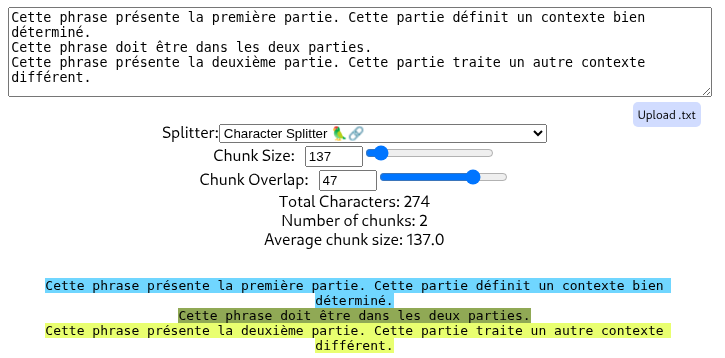
\includegraphics[width=1\linewidth, keepaspectratio]{images/split.png}
\caption{Paramétrage du découpage d'un texte}
\label{fig:split}
\end{figure}
La figure \ref{fig:split} montre comment le chevauchement (texte en vert) est commmun pour les deux chunks: Le premier segment combine le texte en bleu et vert, le deuxième combine le texte en vert et jaune. C'est un exemple illustratif avec les caractères. Néanmoins, dans un découpage réel, le paramétrage dépend de la nature des documents.
Par exemple, pour des PDFs techniques (e.g., manuels ou rapports), une taille de chunk de 300-500 mots avec un chevauchement de 50 mots (10-15\%) préserve les contextes complexes comme les définitions ou les procédures. Pour des articles web courts, une taille de 150-200 mots avec 20-30 mots de chevauchement suffit, assurant une granularité fine sans perte d'information.
\paragraph{Embedding}
 Chaque chunk est transformé en vecteur numérique à l’aide d’un modèle d’embedding (Embbedding Machine dans la figure \ref{fig:embeddings}). 
 % Ce vecteur capture la signification sémantique du texte et permet des recherches par similarité.
\begin{figure}[H]
\centering
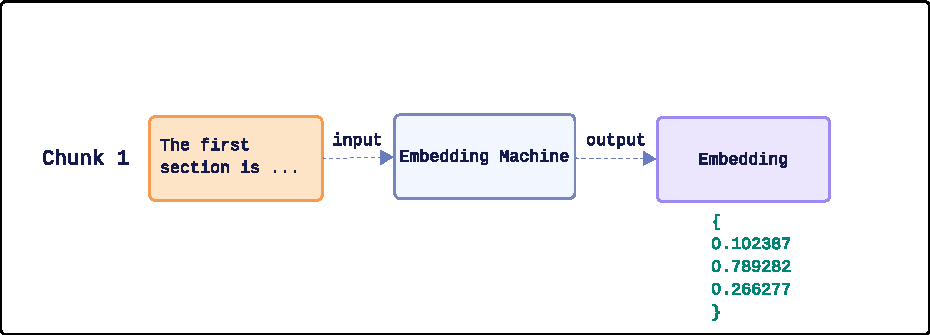
\includegraphics[width=1\linewidth, keepaspectratio]{images/embed_rag.pdf}
\caption{Transformation d'un segment en un vecteur}
\label{fig:embeddings}
\end{figure}
Les embeddings (ou vecteurs denses) sont des représentations numériques de données textuelles, permettant de capturer leur signification sémantique. Au lieu de représenter les mots par des entiers arbitraires ou des identifiants, les embeddings projettent chaque mot, phrase ou document dans un espace vectoriel à plusieurs dimensions. Dans ce nouvel espace, des concepts similaires sont regroupés géométriquement, ce qui permet de mesurer la similarité entre textes à l’aide de distances vectorielles (comme la distance cosinus).\par
La figure suivante démontre un exemple simple en projetant l'espace des vecteurs en 2D: elle illustre la transformation de mots en vecteurs numériques où la proximité géométrique reflète la similarité sémantique. On observe que "cat" et "kitten" sont proches dans l'espace car ils partagent des dimensions félines communes, tandis que le mot "dog" (chien) n'est pas très loin vu que c'est un animal aussi.  En revanche, le mot "houses" (maisons) est très éloigné car il appartient à un domaine sémantique différent. Les paires "man-woman" et "king-queen" forment des relations vectorielles parallèles, montrant comment les embeddings capturent naturellement les analogies linguistiques et les symétries.
\begin{figure}[H]%
    \centering
    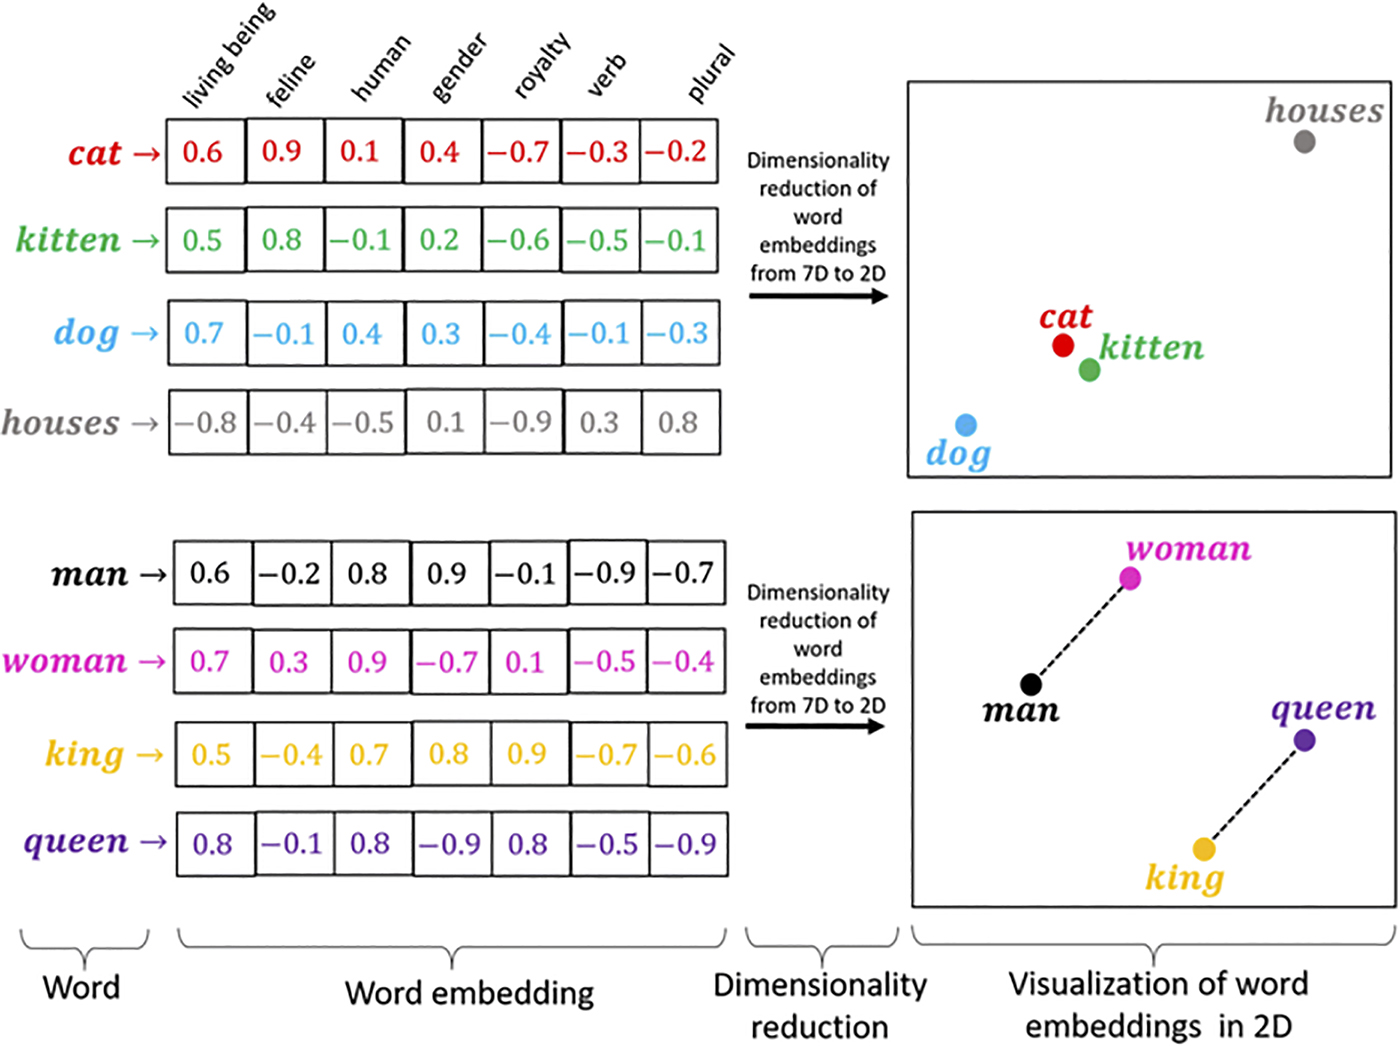
\includegraphics[height=9cm, keepaspectratio]{images/embeddings.jpg}%
    \caption{Les embeddings : transformation en vecteurs et relations sémantiques\cite{laki2022neural}}%
\end{figure}
Les embeddings jouent un rôle fondamental dans les systèmes RAG, car ils permettent d’encoder les documents de la base de connaissance pour les rendre interrogeables efficacement. Lorsqu’un utilisateur envoie une requête, celle-ci est elle-même transformée en embedding, puis comparée à l’ensemble des vecteurs présents dans la base pour retrouver les passages les plus proches sémantiquement.
Il existe plusieurs méthodes pour générer ces vecteurs :
\begin{itemize}[label=\textbullet]
    \item des modèles classiques comme Word2Vec, GloVe ou FastText: basés sur des statistiques de co-occurrence, ils génèrent des vecteurs statiques par mot, idéaux pour des tâches simples comme la classification de texte ou l’analyse de sentiment, mais moins adaptés aux nuances contextuelles.
    \item des modèles contextuels comme BERT ou RoBERTa: utilisant des transformers, ils produisent des vecteurs dynamiques sensibles au contexte, parfaits pour des tâches complexes comme la compréhension de texte ou la traduction, où le sens dépend de l’environnement.
    \item des modèles spécialisés pour la recherche dense, comme OpenAI Ada v2, Cohere ou ceux de la famille SentenceTransformers: optimisés pour la similarité sémantique, ils excellent dans la récupération d’information dans les systèmes RAG, où la précision sur de grands corpus est délicate.
\end{itemize}
Dans notre projet, nous utilisons des embeddings générés par un LLM “text-embedding-3-small” d'OpenAI appartenant à la famille des modèles spécialisés pour la recherche dense, ce qui facilite ainsi une recherche plus fine et appropriée.

\paragraph{Indexation dans une base vectorielle}
 Les vecteurs sont ensuite indexés et stockés dans une base de données vectorielle (Vector Database), qui permet de retrouver efficacement les passages les plus pertinents pour une requête donnée.
\begin{figure}[H]
\centering
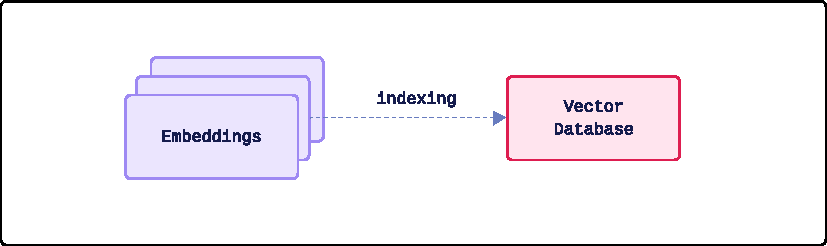
\includegraphics[width=1\linewidth, keepaspectratio]{images/store_rag.pdf}
\caption{Stockage des vecteurs dans la base}
\label{fig:store}
\end{figure}
Une base de données vectorielle (ou vectordb) est une infrastructure conçue pour stocker, indexer et interroger des vecteurs denses. Contrairement aux bases relationnelles traditionnelles, les vectordbs sont optimisées pour la recherche par similarité, en exploitant des techniques comme l’approximate nearest neighbors (ANN), les arbres de partition ou le clustering hiérarchique.\\
Leur rôle est central dans un pipeline RAG : une fois les documents convertis en vecteurs,
ils sont indexés dans la base. Un index, dans ce contexte, est une structure optimisée (comme un arbre ou une grille) qui accélère la recherche en pré-organisant les vecteurs selon leur similarité, réduisant ainsi le temps de comparaison.
Parmi les vectordbs les plus populaires, nous pouvons citer FAISS, Pinecone, Weaviate, Qdrant, Chroma, Milvus ...\\
Nous avons choisi pgvector, une extension légère et extensible de PostgreSQL, pour son intégration fluide dans notre pipeline RAG et ses bonnes performances. Son approche hybride combine la recherche dense (via vecteurs) et lexicale (via texte intégral), surpassant FAISS (limitée à la similarité vectorielle) et Pinecone (SaaS coûteux). De plus, étant open-source, pgvector réduit les coûts par rapport à des solutions SaaS, tout en s’adaptant à notre infrastructure existante.\par
Fonctionnellement, pgvector stocke les vecteurs et le texte brut des chunks dans une table unique. Lors de l’injection, chaque chunk est converti en vecteur et inséré avec son texte ; à la récupération, une requête vectorisée compare les embeddings et retourne directement le texte des chunks les plus proches (top-k), simplifiant le processus sans stockage séparé.
\paragraph{Requête utilisateur et récupération}
Une fois la base de connaissance est prête, l’interaction débute avec la question de l’utilisateur, qui est vectorisée à son tour, puis utilisée pour effectuer une recherche dans la base vectorielle et trouver des passages sémantiquement proches, garantissant qu'ils s’alignent sur le contexte spécifique de la demande.
\begin{figure}[H]
\centering
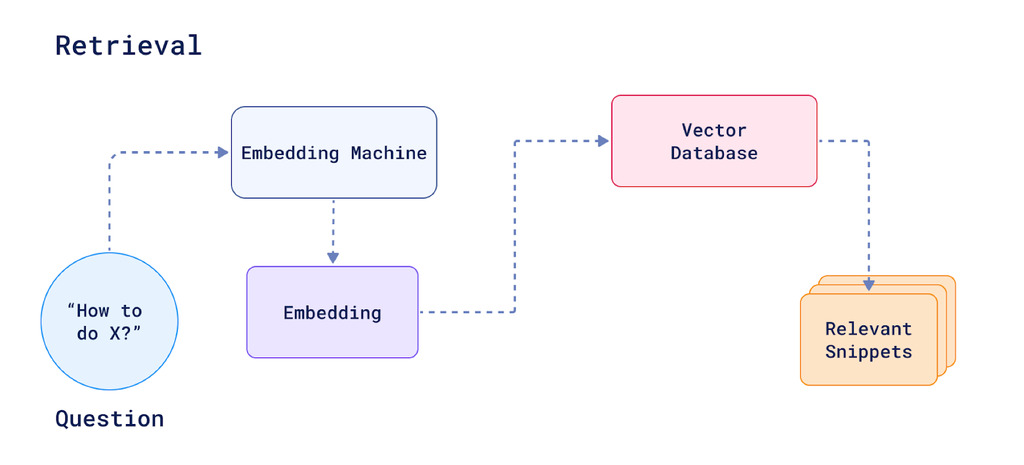
\includegraphics[width=1\linewidth, keepaspectratio]{images/retriever.jpg}
\caption{Phase de récupération \cite{qdrant2024rag}}
\label{fig:retrieve}
\end{figure}
\paragraph{Génération de la réponse}
 Ces passages sélectionnés (Relevant Snippets) sont ensuite injectés dans une requête structurée (prompt) adressée au LLM. Celui-ci utilise à la fois la question de l’utilisateur et les informations extraites pour produire une réponse adaptée. Il ajuste ainsi son raisonnement, évitant les réponses génériques ou hors sujet, et adapte le ton ou le niveau de détail selon les besoins de l’utilisateur. Cette collaboration entre données externes et intelligence du modèle assure une sortie fiable et personnalisée, essentielle pour notre plateforme.
  \begin{figure}[H]
\centering
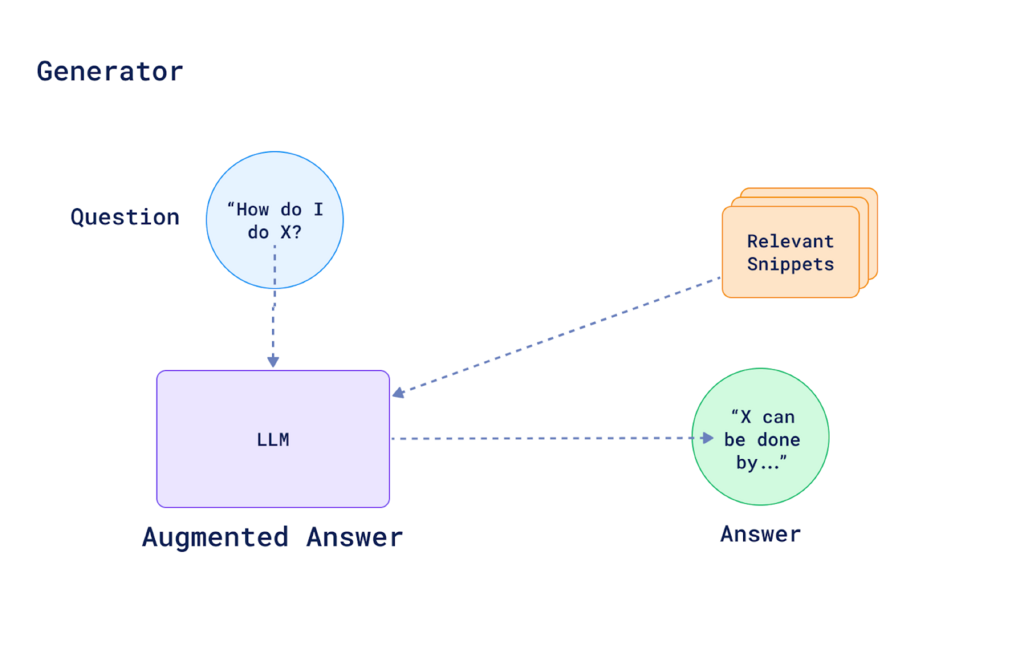
\includegraphics[width=1\linewidth, keepaspectratio]{images/generator.png}
\caption{Phase de génération \cite{qdrant2024rag}}
\label{fig:generate}
\end{figure}
Ce pipeline modulaire peut être optimisé à plusieurs niveaux (qualité des embeddings, stratégie de découpage, méthode de recherche, prompt engineering, etc.), ce qui en fait un terrain riche pour l’expérimentation et l’amélioration continue.

\subsubsection{Optimisations du RAG}
Le pipeline RAG présenté, de nature simple et unitaire, correspond au modèle dit RAG naïf, conçu pour répondre aux exigences fondamentales de notre plateforme en intégrant des données externes par une récupération directe (top-k) à partir d’une base vectorielle. Cette approche est efficace pour des cas d’usage simples, mais ses limites deviennent évidentes face à des contextes complexes ou à des requêtes ambiguës, nécessitant ainsi des ajustements pour garantir des résultats fiables. Afin d’atteindre notre objectif de précision et d’efficacité des réponses, des optimisations avancées ont été explorées.

Ces améliorations peuvent intervenir avant la récupération (pre-retrieval), par exemple à travers le traitement ou l’enrichissement de la requête, ou après la récupération (post-retrieval), comme le re-ranking.
Le re-ranking consiste à réévaluer la pertinence des segments initialement récupérés à l’aide d’un modèle secondaire, tel qu’un cross-encoder, afin d’éliminer les faux positifs et de privilégier les extraits les plus reliés à la requête. D’autres techniques peuvent également renforcer la qualité des résultats. Citons la récupération récursive, qui affine les recherches par itérations successives pour capter des nuances sémantiques, ou encore la génération de résumés, qui transforme des segments volumineux en synthèses claires. Ces approches contribuent à améliorer la précision et l’adaptabilité des réponses face à la diversité des sources.
\begin{figure}[H]%
    \center%
    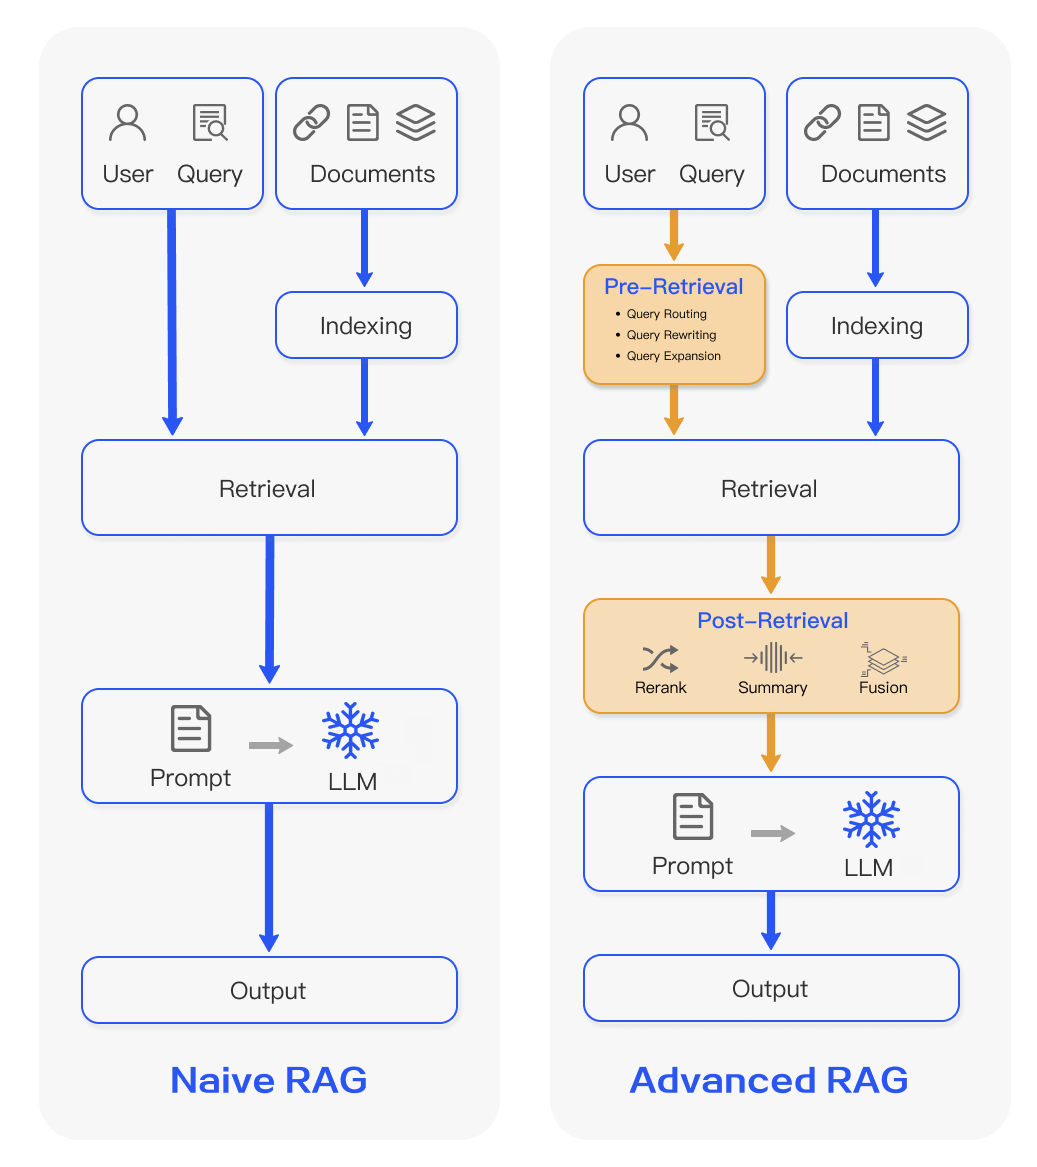
\includegraphics[height=11cm, keepaspectratio]{images/advanced_rag.png}%
    \caption{La différence entre un pipeline naïf et avancé \cite{gao2023retrieval}}%
\end{figure}
Cependant, ces optimisations, bien qu’efficaces, restent centrées sur le pipeline lui-même. Elles atteignent leurs limites lorsque la requête nécessite des ajustements dynamiques ou une orchestration plus flexible des ressources.  
C’est dans ce contexte qu’émerge une approche plus évolutive : le RAG agentique.  
Un agent intelligent, piloté par un modèle de langage, prend en charge le processus. Il adapte les requêtes, oriente la recherche selon la nature des données (exploration vectorielle pour des informations précises ou génération de résumés pour des contenus étendus), et sélectionne les ressources pertinentes, comme des API externes ou une mémoire contextuelle.  
L’agent peut également intervenir dans le découpage des chunks afin d’optimiser la granularité des documents. Cette transition prépare le terrain pour la section suivante, consacrée à l’étude de cette stratégie et à la conception d’assistants modulaires et évolutifs.


\subsection{Les agents}
\subsubsection{Définition}
Les agents \cite{bhide2024building} sont des systèmes qui reposent sur une architecture modulaire où un LLM joue un rôle central dans la prise de décision. Ils sont conçus pour déterminer, organiser et exécuter une série d’actions permettant de répondre à des requêtes complexes. Dans un scénario classique, un agent peut identifier un outil convenable, l’utiliser avec des paramètres spécifiques, analyser sa sortie et enchaîner les étapes jusqu’à fournir une réponse complète à l’utilisateur. Par exemple, face à une demande comme « Réserve-moi un vol et vérifie la météo à destination », un agent peut sélectionner un outil d’API de réservation, calculer les paramètres (dates, lieux), exécuter la recherche, puis utiliser un autre outil météo pour compléter la réponse, tout en analysant les résultats pour assurer une sortie cohérente.
\subsubsection{Composants}
\begin{figure}[H]%
    \center%
    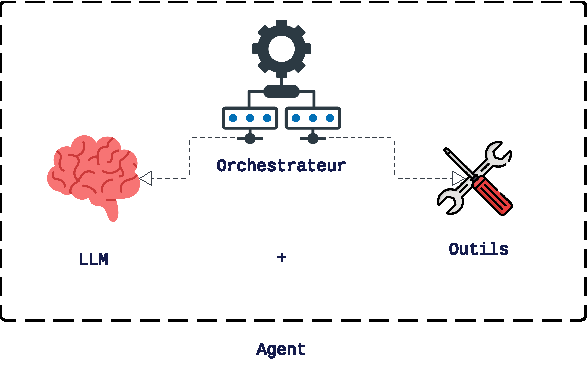
\includegraphics[height=5cm, keepaspectratio]{images/struct_agent.pdf}%
    \caption{Structure générique d'un agent}%
\end{figure}
Un agent se compose généralement de trois éléments fondamentaux:
\begin{itemize}[label=\textbullet]
    \item des outils (tools): Ce sont des ressources opérationnelles permettant d’étendre les capacités du système, incluant des fonctions personnalisées, des API externes (e.g., météo, réservation), des exécutables, ou des services cloud. Ces outils exécutent des traitements spécifiques (e.g., calculs, transformations) ou collectent des données en temps réel (e.g., extraction de texte d’un PDF), offrant ainsi une flexibilité essentielle pour répondre à des requêtes variées.
    \item un moteur de raisonnement (core): Incarné par un LLM, ce composant central analyse la requête, sélectionne les outils appropriés en fonction du contexte (e.g., une API pour une recherche web), interprète leurs sorties (e.g., extrait des données d’une réponse API), et guide les décisions via un raisonnement logique. Il agit comme le cerveau de l’agent, transformant une demande en une séquence d’actions cohérentes.
    \item un orchestrateur: Cette couche clé gère le cycle de décision et la coordination entre le LLM et les outils, assurant un flux d’exécution structuré. Elle définit une logique de boucle itérative : le LLM reçoit une requête initiale, l’orchestrateur intercepte sa sortie (e.g., une instruction comme « Appeler outil X avec paramètres Y »), exécute l’outil correspondant, renvoie le résultat au LLM pour une nouvelle analyse, et répète ce processus jusqu’à atteindre un état de fin (e.g., une réponse finale ou une condition d’arrêt définie). Cette coordination peut être implémentée de plusieurs façons suivant le type de l'agent.
\end{itemize}
\subsubsection{Types d'agents}
On distingue deux grandes familles de comportements :
\paragraph{Agents réactifs}
Ces agents exécutent une action unique ou une séquence linéaire en réponse à une requête. Ils s’appuient souvent sur le paradigme ReAct \cite{yao2023react}, qui combine le raisonnement et l'action pour sélectionner et utiliser un outil (par exemple, une recherche web ou un appel d’API).
\begin{figure}[H]%
\centering
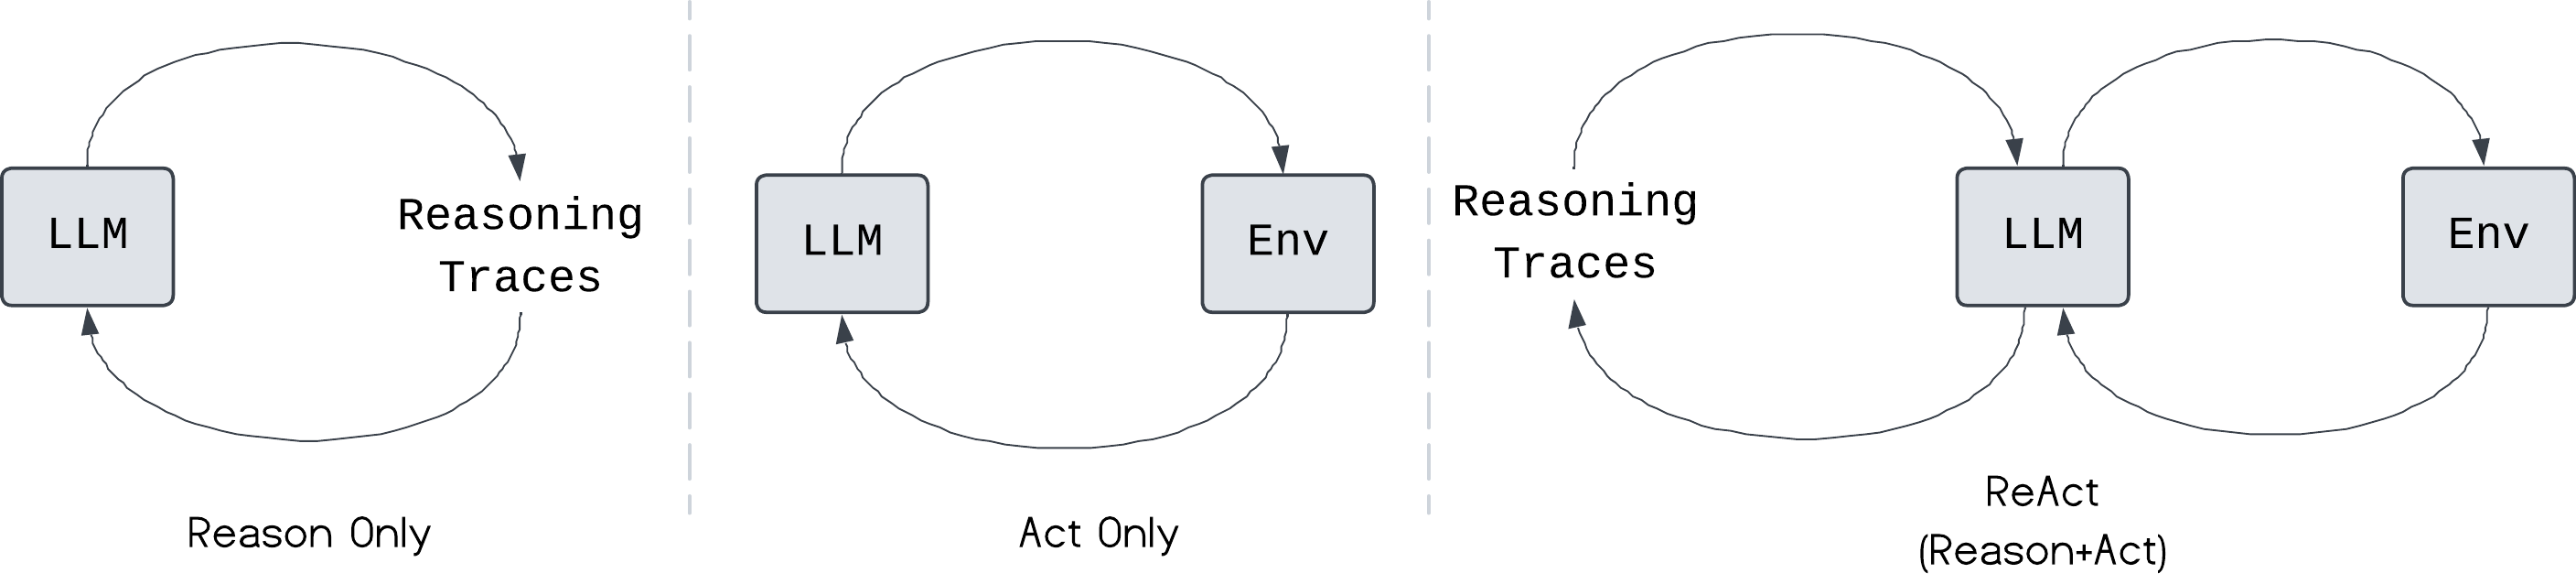
\includegraphics[width=\textwidth, keepaspectratio]{images/react_.png}%
\caption{Agents réactifs}%
\label{fig:react_}
\end{figure}
Comme le montre la figure \ref{fig:react_}, les agents réactifs sont en trois catégories : "Reason Only", "Act Only" et "ReAct (Reason + Act)". L'agent "Reason Only" montre un cycle fermé entre un modèle de langage (LLM) et des traces de raisonnement, indiquant un processus purement introspectif sans interaction externe. L'agent "Act Only" illustre un cycle entre un LLM et un environnement (Env) via des traces, représentant une approche basée uniquement sur l'action sans raisonnement préalable. L'agent "ReAct" combine les deux avec des interactions bidirectionnelles entre le LLM et l'environnement via des traces, reflétant une synergie entre raisonnement et action, essentielle pour une résolution adaptative comme celle observée avec l'exemple suivant.
\begin{figure}[H]%
\centering
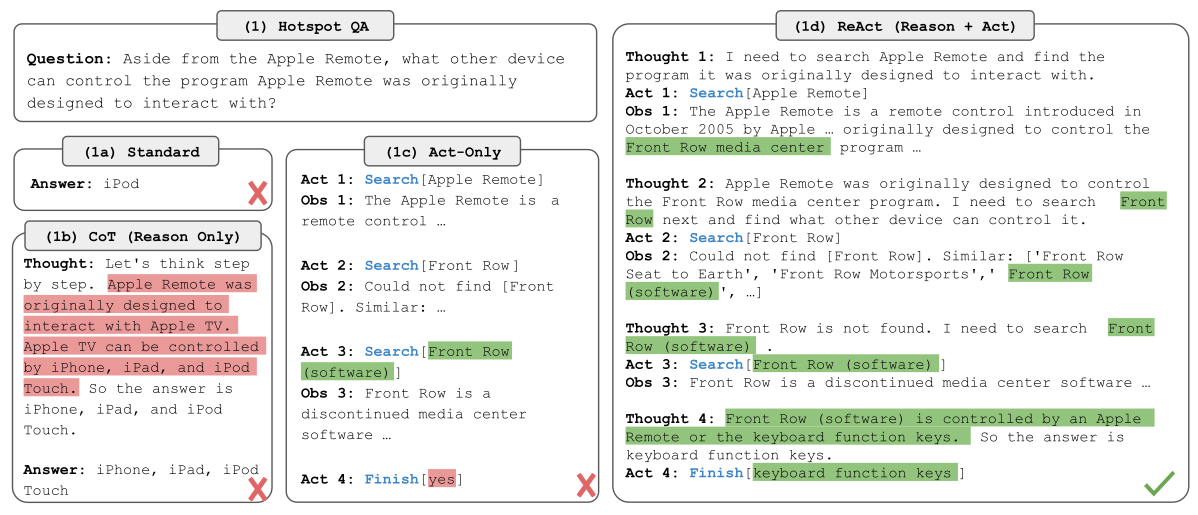
\includegraphics[width=\textwidth, keepaspectratio]{images/react.png}%
\caption{Impacts du paradigme ReAct sur la qualité de réponse \cite{yao2023react}}%
\label{fig:react}
\end{figure}
La figure \ref{fig:react} compare différents types d'agents face à la question sur la compatibilité de l'Apple Remote. L'agent (1a) "Standard" donne une réponse incorrecte (iPod) sans justification. L'agent (1b) "CoT (Reason Only)" raisonne mais n'agit pas, proposant une réponse partielle (iPhone, iPad, iPod Touch) sans confirmation. L'agent (1c) "Act-Only" agit sans raisonnement, échouant à identifier un appareil précis. Enfin, l'agent (1d) "React (Reason + Act)" combine un raisonnement et des actions itératives, recherchant et validant que l'iPhone, iPad et iPod Touch contrôlent Front Row, démontrant une approche réactive et adaptée.

Le fonctionnement de ce type d'agent se base sur une boucle bien gérée par l'orchestrateur:
\begin{figure}[H]%
\centering
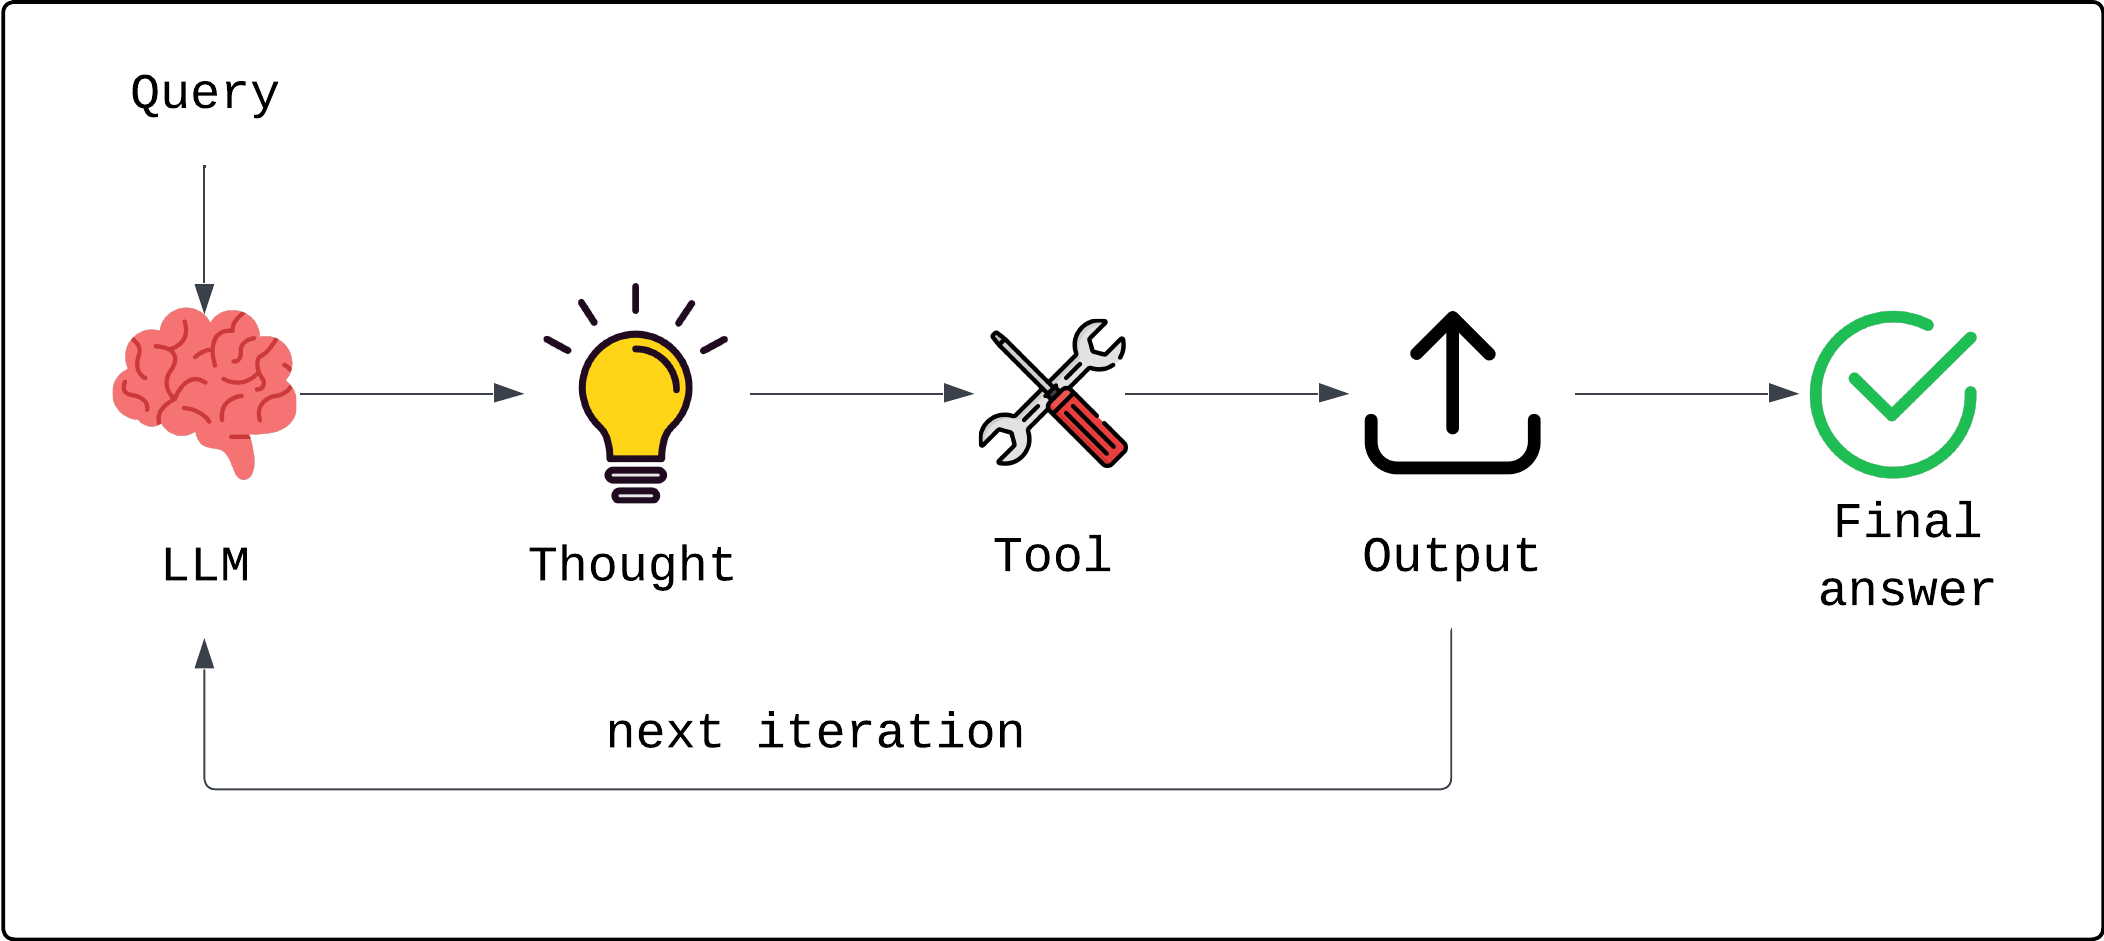
\includegraphics[width=\textwidth, keepaspectratio]{images/react_func.png}%
\caption{Fonctionnement d'un agent ReAct}%
\label{fig:react_func}
\end{figure}
La figure \ref{fig:react_func} illustre le processus d'un agent ReAct. Une requête est initialement traitée par un modèle de langage (LLM), qui génère un raisonnement (Thought). Si nécessaire, un outil (Tool) est utilisé pour obtenir une sortie (Output). Cette sortie est ensuite réintroduite dans le modèle pour une nouvelle itération (next iteration), permettant une observation et un ajustement. Ce cycle se répète jusqu'à ce qu'une réponse finale (Final answer) soit atteinte et validée.
\paragraph{Agents planificateurs} (plan-and-execute agents)
Ces agents décomposent une tâche complexe en un plan structuré, exécutent les actions de manière séquentielle ou parallèle, et ajustent leur stratégie en fonction des résultats. La parallélisation \cite{kim2024llm} des appels de fonctions permet à l’agent d’exécuter simultanément plusieurs tâches indépendantes (par exemple, rechercher des données dans plusieurs sources). Cette optimisation améliore l’efficacité des agents planificateurs, notamment dans des contextes comme le RAG agentique, où la coordination de multiples sources est cruciale.
\begin{figure}[H]%
\centering
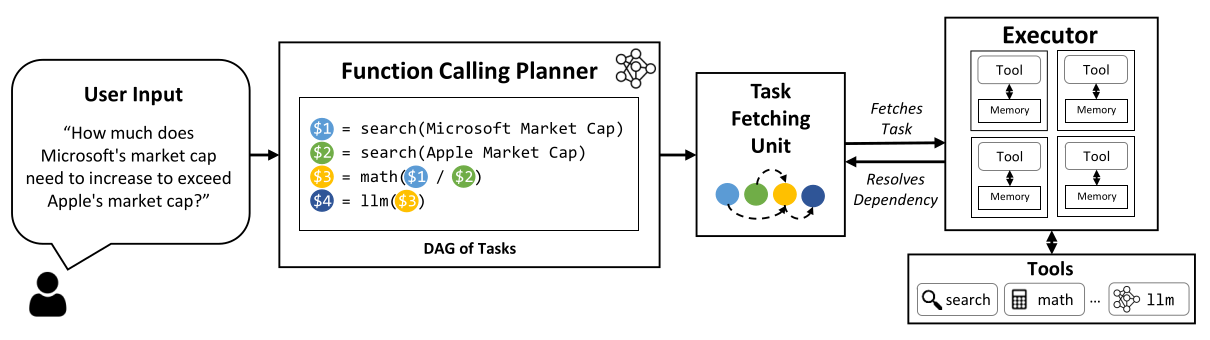
\includegraphics[width=\textwidth, keepaspectratio]{images/compiler.png}%
\caption{Fonctionnement d'un agent planificateur \cite{kim2024llm}}%
\label{fig:compiler}
\end{figure}
La figure \ref{fig:compiler} présente un aperçu de ce type d'agent qui organise les tâches en un graphe orienté acyclique (DAG) avec leurs dépendances. Les tâches sont dispatchées en parallèle par une unité de gestion vers un exécuteur, selon leurs dépendances. Par exemple, les tâches 1 et 2 sont exécutées simultanément pour des recherches indépendantes. Une fois terminées, les résultats sont renvoyés à l'unité de gestion pour débloquer les tâches dépendantes en remplaçant leurs variables (ex. \$1 et \$2 dans la tâche 3) par des valeurs réelles. La réponse finale est ensuite délivrée à l'utilisateur.

Le fonctionnement typique d’un agent peut être résumé ainsi : réception de la requête, sélection éventuelle d’un outil, définition de son entrée, exécution, observation de la sortie, puis répétition du processus jusqu’à l’obtention d’une réponse satisfaisante.
\subsubsection{Typologies des systèmes agentiques}
\begin{figure}[H]%
\centering
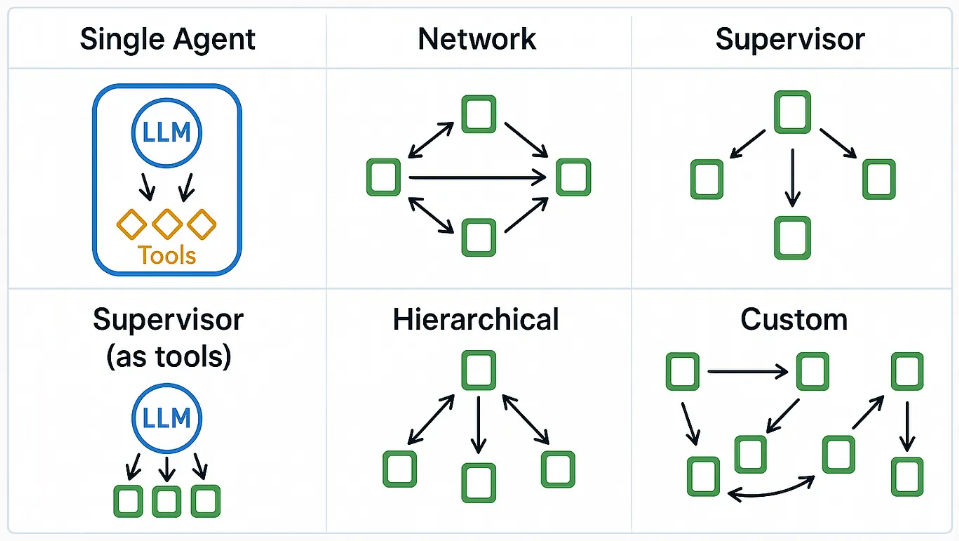
\includegraphics[width=\textwidth, keepaspectratio]{images/agent_typo.png}%
\caption{Typologies et configurations agentiques \cite{agentic_patterns}}%
\label{fig:agent_typos}
\end{figure}

La figure \ref{fig:agent_typos} présente six configurations :
\begin{itemize}[label=\textbullet]
    \item Single Agent : Un modèle de langage (LLM) centralisé utilisant des outils spécifiques pour répondre à une requête.
    \item Network : Une structure où plusieurs agents interagissent de manière bidirectionnelle, collaborant pour résoudre des tâches.
    \item Supervisor : Un agent superviseur coordonne plusieurs agents subordonnés dans une hiérarchie descendante.
    \item Supervisor (as tools) : Un LLM agit comme superviseur, déléguant des tâches à des agents considérés comme des outils.
    \item Hierarchical : Une organisation hiérarchique où un agent principal supervise et distribue des tâches à des agents subordonnés.
    \item Custom : Une configuration personnalisée avec des interactions complexes et des boucles de rétroaction entre agents.
\end{itemize}

Dans notre solution, nous avons exploré diverses de ces configurations pour atteindre notre objectif : une réponse satisfaisante. Nous avons testé plusieurs schémas, ajustant les interactions entre agents dédiés à des tâches spécifiques jusqu'à obtenir un résultat optimal. Cette itération nous a permis de valider l'efficacité d'une architecture adaptée à la complexité de la requête.
\section{Méthodologie adoptée}

Le choix d’une méthode de conduite de projet constitue une étape déterminante. Il permet de garantir la qualité du produit final, de respecter les délais et d’optimiser l’organisation du travail. Pour ce projet, nous avons opté pour une méthode qui fait partie des approches agiles et qui s’adapte particulièrement bien aux environnements dynamiques et évolutifs.
\subsection{Présentation de Scrum}

Scrum \cite{scrum_book} est un cadre méthodologique agile introduit au début des années 1990 pour gérer des projets complexes. Il repose sur le principe d’un développement incrémental et itératif : le produit est construit par étapes successives appelées sprints, d’une durée fixe généralement comprise entre deux et quatre semaines. Chaque sprint aboutit à un incrément fonctionnel, c’est-à-dire une version du produit utilisable.\par

L’un des principaux avantages de Scrum est sa flexibilité : à chaque fin de sprint, l’équipe peut réévaluer les priorités et adapter les fonctionnalités à développer selon les besoins du client. Cette approche favorise donc une meilleure réactivité aux changements pour fournir régulièrement des résultats concrets.\par

Scrum s’appuie sur plusieurs artefacts essentiels :
\begin{itemize}[label=\textbullet]
    \item  Le Backlog Produit (carnet du produit) : la liste des besoins et fonctionnalités à développer, exprimés sous forme de "User Stories".
    \item Le Backlog Sprint (backlog d’itération): les éléments du Backlog Produit sélectionnés pour un sprint donné.
\end{itemize}

\subsection{Rôles dans Scrum}

La méthodologie Scrum définit trois rôles principaux, qui structurent la dynamique de travail :
\begin{itemize}[label=$\triangleright$]
    \item Le Product Owner : représentant du client ou des utilisateurs finaux, il porte la vision du produit et définit les priorités. C’est lui qui alimente et organise le Product Backlog. Dans notre cas, le rôle du Product Owner est joué par Monsieur Omar ABID.
    \item Le Scrum Master : garant de la bonne application de la méthodologie, il facilite la communication et veille à ce que l’équipe reste productive en éliminant les obstacles éventuels. Dans notre cas, le rôle du Scrum Master est joué par Monsieur Omar BACCAR.
    \item L’Équipe de développement : composée de profils techniques, elle est chargée de transformer les besoins exprimés par le Product Owner en fonctionnalités concrètes et testées. Dans le cadre de ce projet, l’équipe était réduite et constituée essentiellement par moi-même.
\end{itemize}

\subsection{Déroulement d’un sprint}

Chaque sprint suit un cycle structuré qui comprend plusieurs étapes :
\begin{itemize}[label={}]
    \item 1. Planification du sprint : réunion initiale au cours de laquelle l’équipe sélectionne, avec le Product Owner, les User Stories à réaliser.
    \item 2. Réunions de suivi (Daily ou Weekly Scrum) : courtes réunions régulières permettant de partager l’avancement, les difficultés rencontrées et les tâches à venir.
    \item 3. Revue de sprint : présentation de l’incrément réalisé au Product Owner et recueil des retours.
    \item 4. Rétrospective : analyse du déroulement du sprint afin d’identifier les points d’amélioration pour la suite.
\end{itemize}
\subsection{Backlog produit}
Le backlog produit recense l’ensemble des besoins identifiés au démarrage du projet. Chaque élément est formulé sous forme de "User Story" afin de rester centré sur la valeur apportée à l'utilisateur final. Le tableau suivant résume le Backlog produit de notre plateforme.
\begin{table}[H]
\centering
\caption{Backlog produit}
\begin{tabular}{|c|p{9cm}|c|}
\hline
\textbf{Id} & \textbf{User story} & \textbf{Priorité}  \\ \hline
A & En tant qu’utilisateur, je souhaite créer, modifier et supprimer un assistant & Élevée \\ \hline
B & En tant qu’utilisateur, je veux créer des conversations et générer des réponses & Élevée  \\ \hline
C & En tant qu’utilisateur, je souhaite tester un assistant (preview) avant de le créer & Moyenne  \\
\hline
D & En tant qu’utilisateur, je veux téléverser des fichiers et générer des embeddings exploitables & Moyenne  \\ \hline
E & En tant qu’utilisateur, je souhaite créer, modifier et supprimer des actions & Élevée \\ \hline
F & En tant qu’utilisateur, je désire gérer des paires de questions/réponses (Les règles de  l'assistant) & Moyenne \\ \hline
\end{tabular}
\end{table}
\subsection{Planification des sprints}
Le projet a été découpé en sprints. Chaque sprint correspond à un incrément fonctionnel livrable, permettant de faire évoluer la plateforme progressivement. Nous les avons mis en place comme le montre le tableau ci-dessous:
% \begin{table}[H]
% \centering
% \begin{tabular}{|c|p{9cm}|c|}
% \hline
% \textbf{Titre} & \textbf{Modules} & \textbf{Durée} \\ \hline
% Sprint 0 & 
% - Étude et analyse des besoins \newline
% - Choix et validation des technologies (frameworks, bases de données, services Azure) \newline
% - Mise en place de l’environnement de développement & 
% 4 semaines \\ \hline

% Sprint 1 & 
% - Développement du microservice de gestion d’assistants (CRUD assistants) \newline
% - Mise en place des endpoints pour créer des conversations et générer des réponses simples & 
% 4 semaines \\ \hline

% Sprint 2 & 
% - Développement du microservice d’upload de fichiers \newline
% - Génération et stockage des embeddings &
% 3 semaines \\ \hline

% Sprint 3 & 
% - Implémentation du microservice orchestrateur pour coordonner les différents services \newline
% - Intégration des fonctionnalités RAG & 
% 4 semaines \\ \hline
% Sprint 4 & 
% - Gestion des actions (CRUD actions) \newline
% - Gestion des paires questions/réponses & 
% 4 semaines \\ \hline
% \end{tabular}
% \caption{Planification des sprints}
% \end{table}

\subsection{Planification des sprints}
Le projet a été découpé en sprints de durée fixe. Chaque sprint correspond à un incrément fonctionnel permettant de faire évoluer la plateforme progressivement. La planification adoptée est présentée dans le tableau ci-dessous :

\begin{table}[H]
\centering
\caption{Planification des sprints}
\begin{tabular}{|c|p{9cm}|c|}
\hline
\textbf{Titre} & \textbf{Modules / Activités} & \textbf{Durée} \\ \hline

Sprint 0 & 
- Étude des besoins et analyse fonctionnelle \newline
- Choix et validation des technologies \newline
- Mise en place de l’environnement de développement & 
3 semaines \\ \hline

Sprint 1 & 
- Développement du microservice de gestion des assistants (CRUD) \newline
- Mise en place des endpoints de base pour les conversations & 
3 semaines \\ \hline

Sprint 2 & 
- Génération de réponses basiques via LLM \newline
- Structuration des flux de conversation & 
3 semaines \\ \hline

Sprint 3 & 
- Développement du microservice d’upload de fichiers \newline
- Génération et stockage des embeddings & 
3 semaines \\ \hline

Sprint 4 & 
- Implémentation du microservice orchestrateur \newline
- Coordination initiale entre les microservices & 
3 semaines \\ \hline

Sprint 5 & 
- Intégration du RAG (récupération top-k depuis la base vectorielle) \newline
- Optimisations et amélioration de la précision des réponses& 
3 semaines \\ \hline

Sprint 6 & 
- Gestion des actions (CRUD actions) \newline
- Gestion des paires questions/réponses & 
3 semaines \\ \hline
\end{tabular}
\end{table}


\section{Conclusion}
Dans ce chapitre, nous avons analysé les solutions existantes et mis en œuvre leurs limites. 
Nous avons ensuite présenté la solution proposée, qui repose sur l’intégration du RAG et d’une approche agentique afin de surmonter les limites des systèmes traditionnels. Finalement, nous avons mentionné la méthodologie de gestion de projet.
Le chapitre suivant sera consacré à l’architecture et à la conception de la plateforme, afin de montrer comment ces principes théoriques ont été traduits en une solution concrète et opérationnelle.